% !TeX root = ../../main.tex

\label{keliyunyi}
在修井作业过程中，井筒内原有颗粒物以及作业过程中产生的新生颗粒物会显著影响井筒工况。颗粒物的存在不仅可能降低井下工具的工作效率，还可能诱发卡钻等重大安全事故。颗粒在井筒内的悬浮状态及运移特性受多种因素共同影响，主要包括颗粒粒径与密度、井眼尺寸与井斜角度，以及洗井液密度、粘度和流速等。本章基于流体动力学与颗粒动力学理论，针对砂砾、铁屑、结垢物和蜡质等典型颗粒物在井筒内的运移规律开展系统研究。通过构建Fluent与EDEM双向耦合仿真模型，定量分析流体参数（流速、粘度）和井筒结构参数（井斜角度）对固体颗粒运移轨迹、沉积速率及空间分布特征的影响规律。

本章仿真方案的具体实施步骤如下：首先，构建颗粒物模型并设置相关参数，基于EDEM平台按照实际物理尺寸完成颗粒注入；其次，构建三维井筒、管柱及环空的几何模型，在Fluent中建立流体仿真模型，设置流体域边界条件；随后，建立Fluent与EDEM之间的双向耦合接口，模拟真实井筒工况下流速、粘度等关键参数对颗粒物运移轨迹、沉积速率及空间分布特征的影响，具体操作流程如图\ref{fig:flowchart}所示；最后，利用后处理模块对仿真结果进行定量分析，包括颗粒分布统计和动力学参数提取。
    \begin{figure}[htbp]
        \centering
        \begin{tikzpicture}[node distance=2cm] % 节点间距为2cm
            % 1. 流场初始化（起始节点）
            \node (init) [startstop] {流场初始化};
            % 2. 连续相流场计算（处理节点）
            \node (flow) [process, below of=init] {连续相流场计算};
            % 3. 颗粒模型注入（处理节点）
            \node (inject) [process, below of=flow] {颗粒模型注入};
            % 4. 颗粒时间步长计算（处理节点）
            \node (time1) [process, below of=inject] {颗粒时间步长计算};
            % 6. 颗粒轨迹计算（处理节点）
            \node (trajectory) [process, below of=time1] {颗粒轨迹计算};
            % 7. 更新连续相源项（处理节点）
            \node (update) [process, below of=trajectory] {更新连续相源项};
            % 8. 判断是否收敛（决策节点）
            \node (converge) [decision, below of=update] {是否收敛};
            % 9. 判断是否计算完成（决策节点）
            \node (complete) [decision, below of=converge] {是否计算完成};
            % 10. 计算结果（终止节点）
            \node (result) [startstop, below of=complete] {计算结果};
            % 11. 更新下一步时间数据（右侧辅助节点）
            \node (nextstep) [process, right of=complete, xshift=4cm] {更新下一步时间数据};

            % 绘制箭头连线
            \draw [arrow] (init) -- (flow);                          % 流场初始化 → 连续相流场计算
            \draw [arrow] (flow) -- (inject);                        % 连续相流场计算 → 颗粒模型注入
            \draw [arrow] (inject) -- (time1);                       % 颗粒模型注入 → 颗粒时间步长计算
            \draw [arrow] (time1) -- (trajectory);                   % 颗粒时间步长计算 → 颗粒轨迹计算
            \draw [arrow] (trajectory) -- (update);                  % 颗粒轨迹计算 → 更新连续相源项
            \draw [arrow] (update) -- (converge);                    % 更新连续相源项 → 判断是否收敛

            % 收敛判断分支（未收敛→返回连续相流场计算）
            \draw [arrow] (converge.west) -- ++(-1,0) |- (flow.west) node[midway, left] {否};

            % 收敛后→计算完成判断
            \draw [arrow] (converge) -- (complete) node [midway, right] {是};

            % 计算完成判断分支（未完成→更新下一步时间数据→返回连续相流场计算）
            \draw [arrow] (complete.east) -- (nextstep.west) node[midway, above] {否};
            \draw [arrow] (nextstep.north) |- (flow.east);

            % 计算完成→输出结果
            \draw [arrow] (complete) -- (result) node[midway, right] {是};
        \end{tikzpicture}
        \caption{颗粒运移模型计算流程图}
        \label{fig:flowchart}  
    \end{figure}

\section{基本理论和模拟条件}  
\subsection{EDEM理论基础} 
井筒中的颗粒在运移过程中产生颗粒-颗粒、颗粒-管壁之间的接触是不可避免的，该过程将产生作用力，本文采用EDEM软件进行模拟。EDEM软件的理论基础是离散元法（Discrete Element Method, DEM），DEM对上述两种接触对进行建模，求解接触中颗粒所受外力作用以及力矩。根据工况的不同，可区分干颗粒和湿颗粒两种类型，
当计算物料为干颗粒时，接触点不存在粘结的作用，EDEM软件默认采用Hertz-Mindlin基本接触模型，颗粒接触受力模型如图\ref{fig:particle_collision}所示。
\begin{figure}[htbp]
	\centering
	\subfloat[双颗粒碰撞模型示意图]{%
		\includegraphics[width=0.45\textwidth]{figure/kelipengzhuang.png}
		\label{fig:particle_collision}
	}
	%\vspace{0pt}
	\subfloat[Hertz--Mindlin 接触模式示意图]{%
		\includegraphics[width=0.55\textwidth]{figure/hertz-mindlin-contact-model.png}
		\label{fig:hertz_mindlin_contact_model}
	}
	\caption{颗粒--颗粒碰撞建模}
	\label{fig:particle_collision_and_contact_model}
\end{figure}

% \begin{figure}[htbp]
% 	\centering
% 	\includegraphics[width=0.6\textwidth]{figure/hertzian-soft-sphere-model.png}
% 	\caption{Hertzian 软球模型}
% 	\label{fig:hertzian_soft_sphere_model}
% \end{figure}


假设发生弹性接触的两球形颗粒的半径分别为 \(R_{1}\)、\(R_{2}\)，则颗粒间产生的法向接触力大小 \(F_{\mathrm{n}}\) 的计算式为
\begin{equation}
	F_{\mathrm{n}}=\frac{4}{3}E_{\mathrm{eq}}\sqrt{R_{\mathrm{eq}}}\,\delta^{3/2}
	\label{eq:normal_particle_elastic_force}
\end{equation}
式中，\(E_{\mathrm{eq}}\) 为等效杨氏模量，$\mathrm{GPa}$；\(\delta\) 为法向重叠量，$\mathrm{mm}$；\(R_{\mathrm{eq}}\) 为等效接触半径，$\mathrm{mm}$。\(E_{\mathrm{eq}}\) 和 \(R_{\mathrm{eq}}\) 的计算式为
\begin{equation}
	\begin{aligned}
		E_{\mathrm{eq}} & = \left(\frac{1 - \nu_1^2}{E_1} + \frac{1 - \nu_2^2}{E_2} \right)^{-1}\\
	R_{\mathrm{eq}} & =\left(\frac{1}{R_{1}}+\frac{1}{R_{2}}\right)^{-1}
	\end{aligned}
\end{equation}
式中，\(E_{1}\)、\(E_{2}\) 分别为颗粒1、2 的杨氏模量，$\mathrm{GPa}$；\( \nu_{1} \)、\( \nu_{2} \) 分别为颗粒 1、2 的泊松比。


颗粒间法向阻尼力 \(F_{\mathrm{n}}^{\mathrm{d}}\) 及切向阻尼力 \(F_{\mathrm{t}}^{\mathrm{d}}\) 的计算公式为
\begin{equation}
	\begin{aligned}
	F_{\mathrm{n}}^{\mathrm{d}} &= 2\sqrt{\frac{5}{6}}\beta\sqrt{S_{\mathrm{n}}m_{\mathrm{eq}}}\,v_{\mathrm{n}}^{\mathrm{rel}}\\
	F_{\mathrm{t}}^{\mathrm{d}} &= 2\sqrt{\frac{5}{6}}\beta\sqrt{S_{\mathrm{t}}m_{\mathrm{eq}}}\,v_{\mathrm{t}}^{\mathrm{rel}}
	\end{aligned}
	\label{eq:normal_shear_damping_force}
\end{equation}
%这是Tsuji阻尼模型
式中，\(S_{\mathrm{n}}\) 为法向刚度，\(S_{\mathrm{t}}\) 为切向刚度，$\mathrm{N/m}$；\(v_{\mathrm{n}}^{\mathrm{rel}}\) 为法向真实速度，\(v_{\mathrm{t}}^{\mathrm{rel}}\) 为切向真实速度，$\mathrm{m/s}$；\(m_{\mathrm{eq}}\) 为等效质量，\(\mathrm{kg}\)；\(\beta\) 为阻尼系数。法向和切向共用同一阻尼系数\(\beta\)，与颗粒碰撞前后的恢复系数\(e\)的关系为
\begin{equation}
	\beta = \frac{\ln e}{\sqrt{\ln^2 e + \pi ^2}}
\end{equation}
%恢复系数e定义为碰撞后法向相对分离速度与碰撞前法向相对接近速度之比：e= v_接近/v_分离

等效质量\(m_\mathrm{eq}\)的计算式为
\begin{equation}
	m_{\mathrm{eq}} = \left(\frac{1}{m_{1}}+\frac{1}{m_{2}}\right)^{-1}	
\end{equation}

\(S_{\mathrm{n}}\) 和\(S_{\mathrm{t}}\)的计算式为
\begin{equation}
	\begin{aligned}
		S_{\mathrm{n}} &= 2E_{\mathrm{eq}}\sqrt{R_{\mathrm{eq}}\delta}\\
		S_{\mathrm{t}} &= 8G_{\mathrm{eq}}\sqrt{R_{\mathrm{eq}}\delta}
	\end{aligned}
\end{equation}

其中，\(G_{\mathrm{eq}}\) 为等效剪切模量，Pa，其计算公式为
\begin{equation}
	G_{\mathrm{eq}}=\left(\frac{2-\nu_{1}}{G_{1}}+\frac{2-\nu_{2}}{G_{2}}\right)^{-1}
\end{equation}
式中，\(G_{1}\)、\(G_{2}\) 分别为颗粒 1、2 的剪切模量。

假设两颗粒产生接触前的速度分别为 \(\bm{v}_{1}\)、\(\bm{v}_{2}\)，\(\bm{n}\) 为产生接触时的法向单位矢量，则
\begin{equation}
		\bm{n}=\frac{\bm{r}_{1}-\bm{r}_{2}}{\left|\bm{r}_{1}-\bm{r}_{2}\right|}
\end{equation}
进而，\(v_{\mathrm{n}}^{\mathrm{rel}}\)和\(v_{\mathrm{t}}^{\mathrm{rel}}\)的计算式为
\begin{equation}
	\begin{aligned}
	v_{\mathrm{n}}^{\mathrm{rel}} &= (\bm{v}_{1}-\bm{v}_{2})\cdot\bm{n} \\
	v_{\mathrm{t}}^{\mathrm{rel}} &= \left|(\bm{v}_{1}-\bm{v}_{2}) - v_{\mathrm{n}}^{\mathrm{rel}}\bm{n} + (\bm{\omega}_{1} \times R_1\bm{n} + \bm{\omega}_{2} \times R_2\bm{n})\right|
	\end{aligned}
\end{equation}

颗粒间的切向力 \(F_{\mathrm{t}}\) 计算式为
\begin{equation}
	F_{\mathrm{t}}=S_{\mathrm{t}}\delta_{\mathrm{t}}
	\label{eq:shear_damping_force}
\end{equation}
%切向方向：接触面没有"几何上的切向重叠"这个概念。两个球在切向方向的相对运动，本质上是接触面发生了弹性剪切变形。这个变形量无法从当前几何位置反推，只能从接触开始的那一刻起，一步步累加相对切向位移。把切向接触想象成一个弹簧-阻尼-滑块串联系统：弹簧：代表接触面的弹性剪切刚度，弹簧的伸长量就是 δt，阻尼器：代表能量耗散，滑块：代表库仑摩擦极限
%这是Mindlin理论
式中，\(\delta_{\mathrm{t}}\)表示两个颗粒的切向重叠量，在两个颗粒建立接触时为零，此后时间步内进行累积
\begin{equation}
	\delta_{\mathrm{t}}^{n+1} = \delta_{\mathrm{t}}^{n} + \Delta t \cdot {v}_\mathrm{t}^\mathrm{rel}
\end{equation}

综合上述，根据式(\ref{eq:normal_particle_elastic_force})和式(\ref{eq:normal_shear_damping_force})，可得颗粒间的法向总接触力 ；根据式子(\ref{eq:normal_shear_damping_force})和式(\ref{eq:shear_damping_force})，可得颗粒间的切向总接触力。当然，切向摩擦力还要收到库伦摩擦定律的限制，在切向总接触里超过静摩擦力（用静摩擦系数\(\mu_s\)进行表征）时进行截断。

% 法向总接触力
\begin{equation}
    \bm{F}_{\mathrm{n}} = F_{\mathrm{n}}\bm{n} + F_{\mathrm{n}}^{\mathrm{d}}\bm{n} = \left(\frac{4}{3}E_{\mathrm{eq}}\sqrt{R_{\mathrm{eq}}}\,\delta^{3/2} + 2\sqrt{\frac{5}{6}}\beta\sqrt{S_{\mathrm{n}}m_{\mathrm{eq}}}\,v_{\mathrm{n}}^{\mathrm{rel}}\right)\bm{n}
    \label{eq:total_normal_force}
\end{equation}

% 切向总接触力（含库仑摩擦截断）
\begin{equation}
    \bm{F}_{\mathrm{t}} = 
    \begin{cases}
        -S_{\mathrm{t}}\bm{\delta}_{\mathrm{t}} - 2\sqrt{\dfrac{5}{6}}\beta\sqrt{S_{\mathrm{t}}m_{\mathrm{eq}}}\,\bm{v}_{\mathrm{t}}^{\mathrm{rel}}, & |\bm{F}_{\mathrm{t}}| \leq \mu_s F_{\mathrm{n}} \\[10pt]
        -\mu_s F_{\mathrm{n}} \dfrac{\bm{v}_{\mathrm{t}}^{\mathrm{rel}}}{v_{\mathrm{t}}^{\mathrm{rel}}}, & |\bm{F}_{\mathrm{t}}| > \mu_s F_{\mathrm{n}}
    \end{cases}
    \label{eq:total_shear_force}
\end{equation}

考虑滚动摩擦提高颗粒运动仿真准确性很重要，接触表面处产生的力矩可以用滚动摩擦系数进行表征，即
% 滚动摩擦扭矩（方向恒定扭矩模型）
\begin{equation}
    \bm{T}_{\mathrm{r}} = -\mu_{\mathrm{r}} F_{\mathrm{n}} R_{\mathrm{eq}} \frac{\bm{\omega}_{\mathrm{rel}}}{|\bm{\omega}_{\mathrm{rel}}|}
    \label{eq:rolling_torque}
\end{equation}
式中，\(\mu_{\mathrm{r}}\) 为滚动摩擦系数；\(\bm{\omega}_{\mathrm{rel}}\) 为接触点的相对角速度，\(\mathrm{rad/s}\)。以上给出了颗粒--颗粒接触碰撞过程的完整建模，对于颗粒--壁面的建模也同理，在此处不在赘述。

当处理湿颗粒且颗粒间存在液桥力等粘性作用时，接触模型通常选用 Hertz--Mindlin with JKR 模型，其法向弹性接触力的计算基于 Johnson--Kendall--Roberts（JKR）理论。
该模型在 Hertz--Mindlin（无滑移）模型的基础上引入了表面能参数，适用于模拟干粉、湿物料等强粘性系统。

JKR 模型的法向力取决于法向重叠量 $\alpha$ 和表面能 $\gamma$，其表达式为：
\begin{equation}
    F_{\mathrm{JKR}}
    = -4\sqrt{\pi\gamma E^{\mathrm{eq}}\alpha^{3}}
    + \frac{4E^{\mathrm{eq}}\alpha^{3}}{3R^{\mathrm{eq}}}
    \label{eq:JKR_force}
\end{equation}

对应的相对接近距离（即法向重叠量）$\delta$ 为：
\begin{equation}
    \delta = \frac{\alpha^{2}}{R^{\mathrm{eq}}}
    - \sqrt{\frac{4\pi\gamma\alpha}{E^{\mathrm{eq}}}}
    \label{eq:JKR_overlap}
\end{equation}

式中：$E^{\mathrm{eq}}$ 为等效杨氏模量；$R^{\mathrm{eq}}$ 为等效半径；$\alpha$ 为考虑粘附力时的接触面半径；$\gamma$ 为表面能（单位：J/m$^{2}$）。

当 $\gamma = 0$ 时，粘附项消失，JKR 法向力退化为经典 Hertz--Mindlin 法向力：
\begin{equation}
    F_{\mathrm{JKR}} = F_{\mathrm{Hertz}}
    = \frac{4}{3}E^{\mathrm{eq}}\sqrt{R^{\mathrm{eq}}}\,\delta^{3/2}
    \label{eq:Hertz_force}
\end{equation}

该模型即使在颗粒未发生物理接触的情况下，仍能提供吸引力（凝聚力）。颗粒间存在非零凝聚力的最大间隙 $\delta_{\mathrm{c}}$ 定义为：
\begin{equation}
    \delta_{\mathrm{c}} = \sqrt[3]{\frac{4\pi\alpha_{\mathrm{c}}}{E^{\mathrm{eq}}}}
    + \frac{\alpha_{\mathrm{c}}^{2}}{R^{\mathrm{eq}}}
    \label{eq:critical_gap}
\end{equation}

其中临界接触半径 $\alpha_{\mathrm{c}}$ 为：
\begin{equation}
    \alpha_{\mathrm{c}} = \left(\frac{9\pi\gamma R^{\mathrm{eq}2}}{2E^{\mathrm{eq}}}\right)^{\frac{1}{3}}
    \label{eq:critical_radius}
\end{equation}

当 $\delta < \delta_{\mathrm{c}}$ 时，模型返回零力。最大凝聚力（即拉脱力，pull-off force）发生在颗粒未实际接触且间隙小于 $\delta_{\mathrm{c}}$ 时，其表达式为：
\begin{equation}
    F_{\mathrm{c}} = -\frac{3}{2}\pi\gamma R^{\mathrm{eq}}
    \label{eq:pull_off_force}
\end{equation}

在实际仿真中，可根据工况调整表面能 $\gamma$ 等参数，以表征不同含水率条件下颗粒的粘性状态。表面能对颗粒流动行为影响显著，含水率越高，所需表面能参数越大。

颗粒间接触采用 EDEM 默认的 Hertz--Mindlin 模型作为基础框架，该模型适用于描述各类形状颗粒（球形、椭球形及不规则颗粒）之间的接触行为，并考虑了颗粒变形、滑移等实际因素。

在采用离散元法进行模拟计算时，通常作如下假设：
\begin{enumerate}
    \item 颗粒被视为刚性或近似刚性实体，形变仅在接触区域以重叠量体现；
    \item 颗粒间接触形式为点接触，接触发生在很小的区域内；
    \item 颗粒间可产生部分重叠，但重叠量远小于颗粒尺寸；
    \item 在每个计算步长内，外力不能同时传播到相邻颗粒，任意颗粒上的合力由其直接接触的颗粒唯一确定。
\end{enumerate}

\subsection{液固相间作用模型}

颗粒在流场中的受力主要分为以下三类：
\begin{enumerate}
	\item 与流体--颗粒相对运动无关的力，包括重力、压力梯度力、浮力等；
	\item 与流体--颗粒相对运动有关，且力的方向沿相对运动方向，包括曳力、虚拟质量力和 Basset 力等；
	\item 与流体--颗粒相对运动有关，且力的方向垂直于相对运动方向，包括 Saffman 力、Magnus 力等。
\end{enumerate}

在液--固两相流的模拟中，正确选择曳力模型有助于提高数值模拟的准确性。常见曳力模型有 Schiller--Naumann 曳力模型、Wen--Yu 曳力模型、Symmetric 曳力模型、Gidaspow 曳力模型、Syamlal--O'Brien 曳力模型等。Gidaspow 曳力模型应用较广，适用于大多数流态化计算，是 Wen--Yu 曳力模型与 Ergun 曳力模型的结合。因此，本文研究主要采用 Gidaspow 曳力模型，如下式所示：
\begin{equation}
	\beta_{\mathrm{Gidaspow}}=
	\begin{cases}
		\dfrac{3C_{\mathrm{d}}\epsilon_{\mathrm{s}}\rho_{\mathrm{l}}\left|\bm{v}_{\mathrm{l}}-\bm{v}_{\mathrm{s}}\right|}{4d_{\mathrm{s}}}\epsilon_{\mathrm{l}}^{-2.65}, & \epsilon_{\mathrm{l}}>0.8 \\[10pt]
		\dfrac{\epsilon_{\mathrm{s}}(1-\epsilon_{\mathrm{l}})\mu_{\mathrm{l}}}{\epsilon_{\mathrm{l}}d_{\mathrm{s}}^{2}}
		+1.75\dfrac{\epsilon_{\mathrm{s}}\rho_{\mathrm{l}}}{d_{\mathrm{s}}}
		\left|\bm{v}_{\mathrm{l}}-\bm{v}_{\mathrm{s}}\right|, & \epsilon_{\mathrm{l}}\leq 0.8
	\end{cases}
\end{equation}
其中，\(C_{\mathrm{d}}\) 为阻力系数，其计算公式如下：
\begin{equation}
	C_{\mathrm{d}}=
	\begin{cases}
		\dfrac{24}{Re_{\mathrm{s}}}\left(1+0.15Re_{\mathrm{s}}^{0.687}\right), & Re_{\mathrm{s}}\leq 1000 \\[8pt]
		0.44, & Re_{\mathrm{s}}>1000
	\end{cases}
\end{equation}

固相雷诺数表示为
\begin{equation}
	Re_{\mathrm{s}}=\frac{d_{\mathrm{s}}\epsilon_{\mathrm{l}}\rho_{\mathrm{l}}
		\left|\bm{v}_{\mathrm{l}}-\bm{v}_{\mathrm{s}}\right|}{\mu_{\mathrm{l}}}
\end{equation}

升力包括剪切升力（Saffman）和旋转升力（Magnus），垂直于颗粒和流体之间的相对速度方向。施加在岩屑颗粒 \(p\) 上的剪切升力（Saffman）表现形式为
\begin{equation}
	\bm{F}_{\mathrm{S}}
	=C_{\mathrm{LS}}\frac{\rho_{\mathrm{l}}\pi}{8}d_{p}^{3}
	\left|\bm{v}_{\mathrm{l}}-\bm{v}_{p}\right|
	\sqrt{\omega_{\mathrm{l}}}
\end{equation}
其中，\(\omega_{\mathrm{l}}\) 为流体速度的旋度，\(C_{\mathrm{LS}}\) 为剪切升力系数，可以表示为
\begin{equation}
	C_{\mathrm{LS}}=\frac{4.1126}{Re_{\mathrm{s}}^{0.5}}f\left(Re_{\mathrm{HB}},Re_{\mathrm{s}}\right)
\end{equation}
\begin{equation}
	f\left(Re_{\mathrm{HB}},Re_{\mathrm{s}}\right)
	=
	\begin{cases}
		\left(1-0.3314\sqrt{\beta}\right)
		e^{-0.1Re_{\mathrm{s}}}
		+0.3314\sqrt{\beta}, & Re_{\mathrm{s}}\leq 40 \\[6pt]
		0.0524\sqrt{\beta Re_{\mathrm{s}}}, & Re_{\mathrm{s}}>40
	\end{cases}
\end{equation}
其中
\begin{equation}
	\beta=\frac{0.5Re_{\mathrm{s}}}{Re_{\mathrm{HB}}},\qquad 0.005<\beta<0.4
\end{equation}

剪切流的雷诺数为
\begin{equation}
	Re_{\mathrm{s}}=\frac{\rho_{\mathrm{l}}d_{p}^{2}\omega_{\mathrm{l}}}{\mu_{\mathrm{l}}}
\end{equation}

作用在颗粒 \(p\) 上的旋转升力（Magnus）的计算公式由 Oesterle 给出：
\begin{equation}
	\bm{F}_{\mathrm{M}}
	=C_{\mathrm{LM}}\frac{\rho_{\mathrm{l}}\pi}{8}d_{p}^{3}
	\left|\bm{v}_{\mathrm{l}}-\bm{v}_{p}\right|
	\frac{\left|\bm{\Omega}\times
		\left(\bm{v}_{\mathrm{l}}-\bm{v}_{p}\right)\right|}
	{\left|\bm{\Omega}\right|}
\end{equation}
其中，\(C_{\mathrm{LM}}\) 为剪切升力系数，可以表示为：
\begin{equation}
	C_{\mathrm{LM}}
	=0.45+\left(\frac{Re_{r}}{Re_{\mathrm{HB}}}-0.454\right)
	\exp\left(-0.5684Re_{r}Re_{\mathrm{HB}}^{-0.3}\right)
\end{equation}

颗粒拟温度的物理意义表示颗粒脉动的脉动能，能够在微尺度上反映颗粒脉动速度的剧烈程度，表征颗粒运动的无序程度，是颗粒相相互碰撞作用以及颗粒相和流体相相互作用的结果。颗粒拟温度的定义为
\begin{equation}
	\theta=\frac{1}{3N}\left[
	\sum_{j=1}^{N}C_{xj}^{2}
	+\sum_{j=1}^{N}C_{yj}^{2}
	+\sum_{j=1}^{N}C_{zj}^{2}
	\right]
\end{equation}

\subsection{液相控制模型}

对于密度恒定的不可压缩流体，假设液相质量为常数，液体流动遵循 N--S 方程。液固两相流模型中流体相的连续性方程和 N--S 方程由下式给出：
\begin{equation}
	\frac{\partial(\rho_{\mathrm{l}}\epsilon_{\mathrm{l}})}{\partial t}
	+\nabla\cdot(\rho_{\mathrm{l}}\epsilon_{\mathrm{l}}\bm{v}_{\mathrm{l}})=0
\end{equation}
\begin{equation}
	\frac{\partial(\rho_{\mathrm{l}}\epsilon_{\mathrm{l}}\bm{v}_{\mathrm{l}})}{\partial t}
	+\nabla\cdot(\rho_{\mathrm{l}}\epsilon_{\mathrm{l}}\bm{v}_{\mathrm{l}}\bm{v}_{\mathrm{l}})
	=-\epsilon_{\mathrm{l}}\nabla P
	-\nabla\cdot(\epsilon_{\mathrm{l}}\bm{\tau}_{\mathrm{l}})
	+\epsilon_{\mathrm{l}}\rho_{\mathrm{l}}\bm{g}+\bm{F}_{p}
\end{equation}
式中，\(\bm{g}\) 为重力加速度，\(\rho_{\mathrm{l}}\) 为流体密度，\(P\) 和 \(\epsilon_{\mathrm{l}}\) 分别为流体相压力和体积分数，\(\bm{v}_{\mathrm{l}}\) 为流体速度，\(\bm{F}_{p}\) 为液固相间作用力，\(\bm{\tau}_{\mathrm{l}}\) 表示粘性应力张量。其中，液固相间作用力及粘性应力张量公式为
\begin{equation}
	\bm{F}_{p}
	=-\frac{\sum_{i=1}^{k_{\mathrm{c}}}\bm{F}_{i,p}}{\Delta V}
\end{equation}
\begin{equation}
	\bm{\tau}_{\mathrm{l}}
	=\mu_{\mathrm{l}}\left[
	\nabla\bm{v}_{\mathrm{l}}
	+\left(\nabla\bm{v}_{\mathrm{l}}\right)^{T}
	\right]
	-\frac{2}{3}\mu_{\mathrm{l}}
	\left(\nabla\cdot\bm{v}_{\mathrm{l}}\right)\bm{I}
\end{equation}
式中，\(\bm{F}_{p}\) 为液体对颗粒 \(p\) 的作用力，\(\mu_{\mathrm{l}}\) 为流体粘度，\(\bm{I}\) 为单位二阶张量。

\subsection{湍流模型}

考虑到高精度、应用简单、计算效率和通用性等需求，本文采用 \(k-\epsilon\) 标准模型作为研究基础来计算钻井液的湍流粘度，其中 \(k\) 为湍流动能，\(\epsilon\) 为耗散率。\(k\) 和 \(\epsilon\) 的输运方程分别表示为：
\begin{equation}
	\frac{\partial}{\partial t}(\rho_{\mathrm{l}}k)
	+\frac{\partial}{\partial x_{i}}(\rho_{\mathrm{l}}kv_{\mathrm{l},i})
	=\frac{\partial}{\partial x_{j}}\left[
	\left(\mu+\frac{\mu_{\mathrm{t}}}{\sigma_{k}}\right)
	\frac{\partial k}{\partial x_{j}}
	\right]
	+G_{k}-\rho_{\mathrm{l}}\epsilon-Y_{\mathrm{M}}
\end{equation}
\begin{equation}
	\frac{\partial}{\partial t}(\rho_{\mathrm{l}}\epsilon)
	+\frac{\partial}{\partial x_{i}}(\rho_{\mathrm{l}}\epsilon v_{\mathrm{l},i})
	=\frac{\partial}{\partial x_{j}}\left[
	\left(\mu+\frac{\mu_{\mathrm{t}}}{\sigma_{\epsilon}}\right)
	\frac{\partial\epsilon}{\partial x_{j}}
	\right]
	+C_{1\epsilon}\frac{\epsilon}{k}
	\left(G_{k}+C_{3\epsilon}G_{b}\right)
	-C_{2\epsilon}\rho_{\mathrm{l}}\frac{\epsilon^{2}}{k}
\end{equation}
式中，\(\rho_{\mathrm{l}}\) 为液相密度，kg/m\(^{3}\)；\(v_{\mathrm{l}}\) 为液相速度，m/s；\(C_{1\epsilon}\)、\(C_{2\epsilon}\)、\(C_{3\epsilon}\) 为常数，且 \(C_{1\epsilon}=1.44\)，\(C_{2\epsilon}=1.92\)。\(\sigma_{k}\) 和 \(\sigma_{\epsilon}\) 分别为 \(k\) 和 \(\epsilon\) 的湍流普朗特数，其取值为 \(\sigma_{k}=1.0\)，\(\sigma_{\epsilon}=1.3\)。\(G_{k}\) 表示由于平均速度梯度产生的湍流动能；\(Y_{\mathrm{M}}\) 表示可压缩湍流脉动膨胀对整体耗散率的影响；\(\mu_{\mathrm{t}}\) 表示湍流粘度系数。\(G_{k}\)、\(Y_{\mathrm{M}}\)、\(\mu_{\mathrm{t}}\) 公式表示如下：
\begin{equation}
	Y_{\mathrm{M}}=2\rho_{\mathrm{l}}\epsilon M^{2}
\end{equation}
\begin{equation}
	\mu_{\mathrm{t}}=\frac{\rho_{\mathrm{l}}C_{\mu}k^{2}}{\epsilon}
\end{equation}

为了模拟井筒内携带颗粒的特性，模型需要通过设计一个环形空间来实现。研究中建立了内径 \(\phi 88.9\) mm、外径 \(\phi 244.475\) mm、\(\phi 177.8\) mm、总长度为 \(1.5\) m 的光滑管柱，用于模拟钻杆（\(3\)-\(1/2'\)）和井筒（\(9\)-\(5/8'\)、\(7'\)），套管和钻杆同心。在模拟过程中，内部钻杆固定，钻井液以一定速度垂直于入口方向流入环形空间，并从另一端出口流出。环空模型如图 1.5、图 1.6 所示。在 EDEM 软件中，颗粒产生于“颗粒工厂”，其初始速度、角速度为零，角度随机。计算采用了非稳态 \(k-\epsilon\) 湍流模型，将颗粒设置为离散相，并利用多面体网格进行建模。边界条件包括速度入口、压力出口，管壁采用无滑移条件。一般计算参数具体数值见表 1.1，重力方向始终竖直向下，对于不同 \(\theta\) 的情况，流体域旋转相应角度。

\begin{figure}[htbp]
	\centering
	\includegraphics[width=0.9\textwidth]{figure/fluid-domain-geometry.png}
	\caption{流体域几何模型示意图}
	\label{fig:fluid_domain_geometry}
\end{figure}

\begin{figure}[htbp]
	\centering
	\includegraphics[width=0.9\textwidth]{figure/fluid-domain-polyhedral-mesh.jpg}
	\caption{流体域多面体单元离散示意图}
	\label{fig:fluid_domain_mesh}
\end{figure}

\begin{table}[H]
	\centering
	\caption{一般计算参数}
	\begin{tabular}{llll}
		\toprule
		名称 & 符号 & 数值 & 单位 \\
		\midrule
		水平井筒长度 & \(L\) & 1.5 & m \\
		井筒直径 & \(D_{\mathrm{H}}\) & 244.475/177.8 & mm \\
		钻杆直径 & \(D_{\mathrm{P}}\) & 88.9 & mm \\
		颗粒密度 & \(\rho_{\mathrm{P}}\) & -- & kg/m\(^{3}\) \\
		洗井液密度 & \(\rho_{\mathrm{l}}\) & -- & kg/m\(^{3}\) \\
		井斜角 & \(\theta\) & 0.0、45.0、90.0 & \(^{\circ}\) \\
		洗井液入口流速 & \(v_{\mathrm{c}}\) & 0.17、0.27、0.37、0.59 & m/s \\
		洗井液粘度 & \(\mu\) & 1.0、1.7 & mPa·s \\
		\bottomrule
	\end{tabular}
\end{table}

在井筒内颗粒物运移特性的研究中，基于对颗粒动力学行为控制作用的大小，选择流体流速 \(v_{\mathrm{c}}\)、流体粘度 \(\mu\) 和井斜角 \(\theta\) 作为主要控制变量。首先，流体流速 \(v_{\mathrm{c}}\) 是决定颗粒悬浮与输运能力的关键参数，流速直接影响流体的动能和湍流强度，进而调控颗粒的启动阈值、悬浮状态及沉积风险。其次，流体粘度 \(\mu\) 通过改变流体的粘滞阻力，显著影响颗粒的沉降速度及与流体的相互作用，高粘度流体可增强颗粒携带能力，但可能增加流动阻力。最后，井斜角 \(\theta\) 作为几何特征的核心变量，通过改变重力在井筒轴线方向的分量，直接影响颗粒的受力平衡：在斜井或水平井中，重力分量的减弱会加剧颗粒沉降的方位选择性，导致非对称沉积。这三个因素共同构成了颗粒运移的“动力--阻力--几何”三元耦合机制，能够系统表征复杂井筒环境下颗粒迁移的物理本质，为优化携粒效率、预测床层形成提供理论支撑。考虑到颗粒属性的不同会对其运移行为产生显著影响，于是，下文分别研究砂砾、铁屑、结垢物和蜡颗粒的运移和分布规律。

\section{井筒内砂砾运移及分布规律研究}

洗井作业中，冲砂工具和管柱的砂堵问题直接影响作业安全与效率。砂堵的本质是砂砾在工具与井筒环空内的异常堆积，其后果不仅限于工具功能失效，例如冲砂液循环中断、卡钻，还会导致非计划停工、设备维修成本攀升。通过仿真研究井筒内工具与井筒环空砂砾运移规律，可以预测砂砾在井筒环空内的运移速度以及沉积规律，为冲砂作业提供理论指导。

根据现场提供的砂砾样本（见图 1.7）及其粒度分级统计数据（参见表 0.2），建立相对应的大小与数量的砂砾颗粒仿真模型（具体参数见表 0.3）。

\begin{figure}[htbp]
	\centering
	\includegraphics[width=0.5\textwidth]{figure/sand-sample.jpg}
	\caption{井筒出砂样本}
	\label{fig:sand_sample}
\end{figure}

\begin{table}[H]
	\centering
	\caption{砂砾粒度分级统计}
	\begin{tabular}{lll}
		\toprule
		分类 & 粒级区间/\(\mu\)m & 含量/\% \\
		\midrule
		砾石 & \(\leq 2000\) & 0.00 \\
		巨砂 & 2000.00--1000.00 & 0.00 \\
		粗砂 & 1000.00--500.00 & 1.03 \\
		中砂 & 500.00--250.00 & 35.29 \\
		细砂 & 250.00--125.00 & 47.15 \\
		极细砂 & 125.00--62.50 & 13.99 \\
		粗粉砂 & 62.50--31.25 & 1.92 \\
		细粉砂 & 31.25--3.90 & 0.61 \\
		粘土 & \(\leq 3.90\) & 0.00 \\
		\bottomrule
	\end{tabular}
\end{table}

\begin{table}[H]
	\centering
	\caption{仿真颗粒粒径及数量分布}
	\begin{tabular}{llll}
		\toprule
		类型 & 砂砾颗粒数量/个 & 粒径分布比例/\% & 粒径大小/\(\mu\)m \\
		\midrule
		粗砂 & 1000 & 1.0 & 750 \\
		中砂 & 35000 & 35.0 & 375 \\
		细砂 & 47000 & 47.0 & 187.5 \\
		极细砂 & 14000 & 14.0 & 93.75 \\
		粗粉砂 & 2000 & 3.0 & 46.875 \\
		\bottomrule
	\end{tabular}
\end{table}

本项目涉及到的四类工具中，“四合一”工具的外部功能单元多，结构最为复杂，在工具的几何变径处会产生边界层分离和回流现象，是砂砾沉积的“危险位置”。于是，本文选择“四合一”工具的扶正器和强磁位置作为对象，研究砂砾在此处的沉积行为。建立强磁部位与 \(7'\) 井筒环空流体仿真模型，仿真模型数据见表 1.4。研究不同环空流速下（\(v_{\mathrm{c}}=0.37\) m/s、\(0.59\) m/s）砂砾的运移及沉降规律，探究砂砾是否会出现沉积或者堵塞现象。计算结果如图 1.8 所示。

\begin{table}[H]
	\centering
	\caption{“四合一”工具砂砾沉积仿真模型数据}
	\begin{tabular}{llll}
		\toprule
		名称 & 符号 & 数值 & 单位 \\
		\midrule
		水平井筒长度 & \(L\) & 1.5 & m \\
		井筒直径 & \(D_{\mathrm{H}}\) & 177.8 & mm \\
		钻杆直径 & \(D_{\mathrm{P}}\) & 88.9 & mm \\
		颗粒密度 & \(\rho_{\mathrm{P}}\) & 2650.0 & kg/m\(^{3}\) \\
		洗井液密度 & \(\rho_{\mathrm{l}}\) & 1000.0 & kg/m\(^{3}\) \\
		井斜角 & \(\theta\) & 90.0 & \(^{\circ}\) \\
		洗井液入口流速 & \(v_{\mathrm{c}}\) & 0.37、0.59 & m/s \\
		洗井液粘度 & \(\mu\) & 1.0 & mPa·s \\
		\bottomrule
	\end{tabular}
\end{table}

\begin{figure}[htbp]
	\centering
	\includegraphics[width=\textwidth]{figure/tool-and-wellbore-simulation-model.png}
	\caption{工具及井筒仿真模型}
	\label{fig:tool_wellbore_model}
\end{figure}

图 1.9 描述的是洗井液流速 \(0.37\) m/s 下井筒与工具环空内砂砾颗粒分布情况。从图可以看出，部分砂砾颗粒由于重力作用会在工具前端产生堆积，同时砂砾颗粒会随着工具的导流结构进行运移，在强磁部件的凹槽内也会有少量的砂砾堆积现象。

\begin{figure}[htbp]
	\centering
	\includegraphics[width=\textwidth]{figure/sand-distribution-tool-vin-dot37.png}
	\caption{洗井液流速 0.37 m/s 下井筒与工具环空内砂砾颗粒分布}
	\label{fig:sand_distribution_tool_vin_dot37}
\end{figure}

图 1.10 描述的是相同时间步环空流速 \(0.37\) m/s、\(0.59\) m/s 下砂砾颗粒分布。从图中可以看出，环空流速增大时，靠近压力出口的砂砾颗粒越多，砂砾颗粒的运移效率明显加快。在相同时间步下，环空流速越大，颗粒运移速度越快。由于环空流速增大，流体的拖曳力增大，砂砾颗粒在轴向的速度增大，砂砾颗粒由于重力作用产生的沉积位置与流体入口的距离也变远。

\begin{figure}[htbp]
	\centering
	\subfloat[环空流速 0.37 m/s]{%
		\includegraphics[width=0.98\textwidth]{figure/sand-distribution-annular-vin-dot37.png}
		\label{fig:sand_distribution_annular_vin_dot37}
	}
	\vspace{0pt}
	\subfloat[环空流速 0.59 m/s]{%
		\includegraphics[width=0.98\textwidth]{figure/sand-distribution-annular-vin-dot59.png}
		\label{fig:sand_distribution_annular_vin_dot59}
	}
	\caption{相同时间步不同环空流速下砂砾颗粒分布}
	\label{fig:sand_distribution_annular_vin}
\end{figure}

通过仿真发现，在冲砂作业时，如果环空流体中砂砾体积分数越大，越容易在工具与井筒下壁之间的环空中产生沉积，环空流速增大，砂砾运移效率加快，建议在作业时增大洗井液流速即增大冲砂液排量以减小砂砾堆积的风险，降低砂堵概率。同时，工具的导流结构也对砂砾运移起到关键作用，砂砾颗粒会随着工具的导流结构进行运移，降低了砂堵的风险，为工具安全作业提供保障。

上述研究仅仅从宏观上观测砂砾在井筒环空中的运移情况，无法提取井筒环空中不同具体位置的砂砾体积分数、砂砾速度及砂砾床厚度等数据。为此，本研究考虑井筒环空不同位置的砂砾量，基于欧拉液固两相流模型和 \(SST k-\omega\) 模型，建立了三维井眼环空颗粒运移模型，在分析砂砾体积分数和砂砾速度的基础上，通过 Fluent 分析整个环空中砂砾质量，提出了环空内含有颗粒质量的变化方法，分析了幂律流体中环空流速、井斜角度、洗井液粘度等对环空内沉降的砂床高度的影响。所得结论对水平井和大位移井环空内井筒清洁和高效作业具有指导意义。

\subsection{数值模型建立}

根据实际工况，在钻井过程中，钻井液携带砂砾颗粒进入环空，因此内部环境为复杂的液--固两相流湍流流场，故选用 Eulerian 两相流模型对环空砂砾运移进行数值模拟，将环空流场视为稳定的不可压缩湍流流场。

\subsubsection{幂律流体}

钻井液属于非牛顿流体，其本构方程符合幂律流体，流变参数
\begin{equation}
	\tau=K\dot{\gamma}^{n}
\end{equation}
其中，\(K\) 为钻具内钻井液稠度系数，\(n\) 为钻井液流变指数。依据相关文献，\(K=2.38\)，\(n=0.80\)。

\subsection{几何模型及边界条件}

\subsubsection{几何模型}

根据现场实际油井组合参数建立环空三维模型，如图 1.11 所示。实际水平井段很长，为了研究方便，取水平井模型长 \(1.5\) m，取曲率半径 \(1\) m、曲率为 \(90^{\circ}\) 的圆弧弯管模型模拟不同井斜角度，考虑井壁和钻杆表面光滑，计算流域由钻杆和井壁表面组成。采用多面体单元对所建模型进行网格划分。

\begin{figure}[htbp]
	\centering
	\includegraphics[width=0.8\textwidth]{figure/annular-3d-model.png}
	\caption{环空三维模型}
	\label{fig:annular_3d_model}
\end{figure}

\subsubsection{边界条件}

考虑模拟运算中的收敛性和稳定性，湍流流场的计算采用二阶迎风格式和 SIMPLE 算法。根据实际工况对模型入口边界条件定义，具体为：洗井液速度入口和砂砾颗粒入口；出口边界条件为 outlet；将井壁与钻杆表面设为 stationary wall。具体模拟参数如下：井眼直径 244.475 mm，钻杆直径 88.9 mm，砂砾密度 \(2650\) kg/m\(^{3}\)，洗井液密度 1000、1300、1400 kg/m\(^{3}\)，砂砾直径 250 \(\mu\)m，钻井液入口排量 25、40、100 m\(^{3}\)/h，洗井液粘度为 1、2.3、5 cp。

\subsection{数值模拟及结果分析}

\subsubsection{环空砂砾沉降分析}

通过对井筒环空内砂砾质量进行仿真，得到钻杆静止时环空内砂砾沉降质量变化曲线，如图 1.12 所示。由图可知，环空内砂砾质量曲线先呈线性增长，在 30 s 后不再继续增长，而是随时间在稳定值上下波动。这说明井筒内进入的砂砾量与出口排出的砂砾量接近，可判断环空内沉积的砂砾量达到稳定值，平均岩屑质量为 \(63.294\) kg。

\begin{figure}[htbp]
	\centering
	\includegraphics[width=0.7\textwidth]{figure/sand-mass-in-annular-VS-time.png}
	\caption{环空内砂砾质量变化曲线}
	\label{fig:sand_mass_in_annular_VS_time}
\end{figure}

图 1.13 和图 1.14 分别为不同位置截面砂砾轴向速度云图和砂砾体积分数云图。其中水平段每个截面间距 \(500\) mm，井斜段井斜角度间隔 \(15^{\circ}\)，且距离入口 500、1000、1500 mm 处，井斜段 \(15^{\circ}\)、\(30^{\circ}\)、\(75^{\circ}\) 处截面进行放大。环空中砂砾量达到稳定后，由于整个环空中的砂砾不是均匀分布，所以不同位置砂砾速度和体积分数有一定差异。由图可知：环空上部为流体高速区，流速大；下部为低速区，流速趋近于 0。由于重力作用，砂砾趋向环空下部，大部分砂砾沉降在环空下部低速区，造成砂砾难以运移，最终形成砂砾床。

\begin{figure}[htbp]
	\centering
	\includegraphics[width=0.8\textwidth]{figure/sand-velocity-cloud-sections.png}
	\caption{不同截面砂砾速度云图}
	\label{fig:sand_velocity_cloud_sections}
\end{figure}

\begin{figure}[htbp]
	\centering
	\includegraphics[width=0.8\textwidth]{figure/sand-volume-fraction-cloud-sections.png}
	\caption{不同截面砂砾体积分数云图}
	\label{fig:sand_volume_fraction_cloud_sections}
\end{figure}

\subsubsection{洗井液流速对环空砂砾沉积的影响}

图 1.15 为粘度 \(2.3\) cp，排量 25、40、100 m\(^{3}\)/h（0.17、0.27、0.69 m/s）时，不同流速下环空内砂砾质量随时间的变化曲线。由图可以看出，随着时间的延长，环空内沉降的砂砾质量趋于稳定，并且随着流速升高，环空内沉降的砂砾质量减小，且到达稳定的时间加快。

\begin{figure}[htbp]
	\centering
	\includegraphics[width=0.7\textwidth]{figure/sand-mass-in-annular-VS-time-flowrate.png}
	\caption{不同流速下环空内砂砾质量随时间的变化曲线}
	\label{fig:sand_mass_in_annular_VS_time_flowrate}
\end{figure}

假设环空内体积分数最大且沉积高度最高的位置为最容易发生砂堵位置，定为 block 点（简称 b 点）。图 1.16 为流速为 \(0.17\) m/s 时环空内砂砾的体积分数云图，则流速为 \(0.17\) m/s 时，b 点出现在水平段距离入口 \(1280\) mm 处，高度为 \(68\) mm。砂砾床主要沉积在水平段，随着井斜角度增加，砂砾体积分数逐渐减小，井斜 \(75^{\circ}\) 时，砂砾体积分数接近于 0。

\begin{figure}[htbp]
	\centering
	\includegraphics[width=0.7\textwidth]{figure/sand-volume-fraction-vin-dot17.png}
	\caption{流速为 0.17 m/s 时环空内砂砾的体积分数云图}
	\label{fig:sand_volume_fraction_vin_dot17}
\end{figure}

图 1.17 为流速为 \(0.27\) m/s 时环空内砂砾的体积分数云图，流速为 \(0.27\) m/s 时，b 点出现在水平段距离入口 \(1150\) mm 处，高度为 \(64\) mm。砂砾床主要沉积在水平段，相对于 \(0.17\) m/s 流速工况，砂砾在井斜段体积分数有所增加，砂砾向出口运移的效率增大。

\begin{figure}[htbp]
	\centering
	\includegraphics[width=0.7\textwidth]{figure/sand-volume-fraction-vin-dot27.png}
	\caption{流速为 0.27 m/s 时环空内砂砾的体积分数云图}
	\label{fig:sand_volume_fraction_vin_dot27}
\end{figure}

图 1.18 为流速为 \(0.69\) m/s 时环空内砂砾的体积分数云图，流速为 \(0.69\) m/s 时，b 点出现在水平段距离入口 \(1530\) mm 处，高度为 \(32\) mm。砂砾床沉积在水平段及小倾角井斜段，砂砾床高度明显降低，砂堵风险明显下降，且井斜段砂砾体积分数明显增大，砂砾运移效率增大。

\begin{figure}[htbp]
	\centering
	\includegraphics[width=0.7\textwidth]{figure/sand-volume-fraction-vin-dot69.png}
	\caption{流速为 0.69 m/s 时环空内砂砾的体积分数云图}
	\label{fig:sand_volume_fraction_vin_dot69}
\end{figure}

图 1.19 为 b 点高度随洗井液流速变化曲线，由图中可以看到随着洗井液流速增大，b 点高度逐渐减小。

\begin{figure}[htbp]
	\centering
	\includegraphics[width=0.7\textwidth]{figure/b-point-height-VS-flowrate.png}
	\caption{b 点高度随洗井液流速变化曲线}
	\label{fig:b_point_height_VS_flowrate}
\end{figure}

图 1.20 为 b 点不同洗井液流速下砂砾体积分数和轴向速度云图，随着洗井液流速增大，b 点砂砾体积分数减小，且砂砾流速增大，这说明环空排量的增大，增强了流体的携砂能力，促进了砂砾颗粒在环空中的流动性，增加了砂砾颗粒能量，为砂砾运移提供了更大的拖曳力，从而有效地提高了井筒内砂砾颗粒的运移效率。因此在实际作业中，要想减小砂堵风险，宜尽量采用更大的冲砂排量。

\begin{figure}[htbp]
	\centering
	\includegraphics[width=0.8\textwidth]{figure/sand-volume-fraction-velocity-at-b-point-flowrate.png}
	\caption{b 点不同洗井液流速下砂砾体积分数和轴向速度云图}
	\label{fig:sand_volume_fraction_velocity_at_b_point_flowrate}
\end{figure}

\subsubsection{洗井液粘度对环空砂砾沉积的影响}

图 1.21 为流速 \(0.27\) m/s 时，粘度分别取 1.0、2.3、5.0 cp 时，不同粘度下环空内砂砾质量随时间的变化曲线。由图可以看出，随着时间的延长，环空内沉降的砂砾质量趋于稳定，并且随着粘度增大，环空内沉降的砂砾质量减小，且到达稳定的时间加快。

\begin{figure}[htbp]
	\centering
	\includegraphics[width=0.7\textwidth]{figure/sand-mass-in-annular-VS-time-viscosity.png}
	\caption{不同粘度下环空内砂砾质量随时间的变化曲线}
	\label{fig:sand_mass_in_annular_VS_time_viscosity}
\end{figure}

图 1.22 为粘度为 \(1.0\) cp 时环空内砂砾的体积分数云图，则粘度为 \(1.0\) cp 时，b 点出现在水平段距离入口 \(800\)--\(1400\) mm 处，高度为 \(77.5\) mm。砂砾床主要沉积在水平段，随着井斜角度增加，砂砾体积分数逐渐减小，井斜 \(75^{\circ}\) 时，砂砾体积分数接近于 0。

\begin{figure}[htbp]
	\centering
	\includegraphics[width=0.7\textwidth]{figure/sand-volume-fraction-mu-1cp.png}
	\caption{粘度为 1.0 cp 时环空内砂砾的体积分数云图}
	\label{fig:sand_volume_fraction_mu_1cp}
\end{figure}

图 1.23 为粘度为 \(5.0\) cp 时环空内砂砾的体积分数云图，则粘度为 \(5.0\) cp 时，b 点出现在水平段距离入口 \(1000\) mm 处，高度为 \(25\) mm。砂砾床沉积在水平段及小倾角井斜段，砂砾床高度明显降低，砂堵风险明显下降，且井斜段砂砾体积分数明显增大，砂砾运移效率增大。

\begin{figure}[htbp]
	\centering
	\includegraphics[width=0.7\textwidth]{figure/sand-volume-fraction-mu-5cp.png}
	\caption{粘度为 5.0 cp 时环空内砂砾的体积分数云图}
	\label{fig:sand_volume_fraction_mu_5cp}
\end{figure}

图 1.24 为 b 点高度随洗井液粘度变化曲线，由图中可以看到随着洗井液粘度增大，b 点高度逐渐减小。

\begin{figure}[htbp]
	\centering
	\includegraphics[width=0.7\textwidth]{figure/b-point-height-VS-viscosity.png}
	\caption{b 点高度随洗井液粘度变化曲线}
	\label{fig:b_point_height_VS_viscosity}
\end{figure}

图 1.25 为 b 点不同洗井液粘度下砂砾体积分数和轴向速度云图，随着洗井液粘度增大，b 点砂砾体积分数减小，但砂砾流速有减小的趋势，这说明洗井液粘度的增大，增大了流体的携砂能力，但是会减小环空中流体的流动性，这说明增大洗井液粘度可以抑制砂堵在井底的形成，但是也会增加砂砾上返的时间。因此在实际作业中，要想减小砂堵风险，宜采用粘度更大的洗井液。

\begin{figure}[htbp]
	\centering
	\includegraphics[width=0.8\textwidth]{figure/sand-volume-fraction-velocity-at-b-point-viscosity.png}
	\caption{b 点不同洗井液粘度下砂砾体积分数和轴向速度云图}
	\label{fig:sand_volume_fraction_velocity_at_b_point_viscosity}
\end{figure}

\section{井筒内铁屑运移及分布规律}
%20260704想法：仿真->实验->外推。这个研究属于“基础性研究”（与4.适用条件中“拓深技术理论及基础性研究”对应），界定了研究的性质——是基础理论研究，不是工程应用。目的是“揭示影响工具应用效果的主控因素”，对应5.1.2 ①的要求是“研究不同流速、粘度、井斜下的运移规律”，通过实验验证哪些参数是影响运移的“主控因素”（Re（实验已经证明）、井斜角的影响在全井筒模型实验中展示）。

在井下封隔器套铣作业过程中，将产生包含多种形态碎屑的混合物（见图\ref{fig:iron_shavings_sample}），其中，金属碎屑（尤其是铁屑）不仅可能导致筛管堵塞风险，还可能导致工具活动部件卡滞。经磨铣封隔器作业上返的碎屑样本分析表明，金属碎屑主要包含环状颗粒、块状颗粒及丝状颗粒三种形态。其中，丝状铁屑因其特有的几何特征，易通过旋转与缠绕作用形成网状结构，从而显著提升孔隙滞留概率。该类颗粒的高长径比特性不仅加剧了运移过程的复杂性，其各向异性运动模式及增大的比表面积更强化了流体拖曳力与壁面吸附效应，为油井金属碎屑对流动通道的动态阻塞机制提供了更真实的物理表征。基于上述特性分析，本研究选取丝状铁屑作为典型颗粒开展建模研究，具体模型及参数见图\ref{fig:iron_particle_comparison}和表\ref{tab:simulation_params}。

\begin{figure}[htbp]
    \centering
    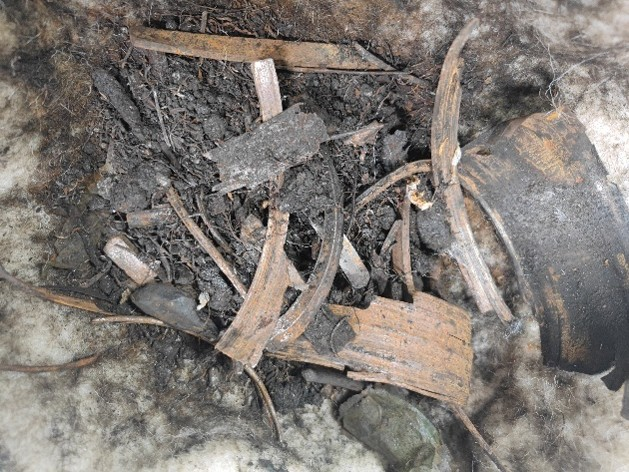
\includegraphics[width=0.5\textwidth]{figure/iron-shavings-sample.jpg}
    \caption{井下封隔器套铣作业中产生的金属碎屑样本}
    \label{fig:iron_shavings_sample}
\end{figure}

\begin{figure}[htbp]
    \centering
    % 子图 (a)
    \subfloat[实际铁屑颗粒]{%
        \begin{minipage}[t]{0.48\linewidth}
            \centering
            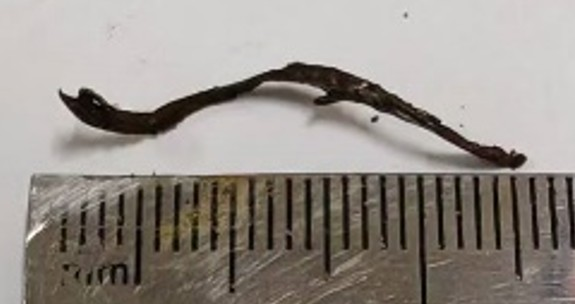
\includegraphics[width=\linewidth]{figure/iron-wire-actual.jpg}
            \label{fig:actual}
        \end{minipage}%
    }
    \hfill
    % 子图 (b)
    \subfloat[铁屑颗粒模型]{%
        \begin{minipage}[t]{0.45\linewidth}
            \centering
            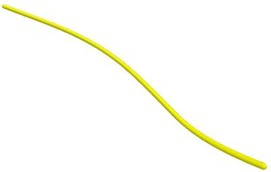
\includegraphics[width=\linewidth]{figure/iron-wire-model.jpg}
            \label{fig:model}
        \end{minipage}%
    }
    % 总标题
    \caption{铁屑颗粒及仿真模型}
    \label{fig:iron_particle_comparison}
\end{figure}

\begin{table}[htbp]
    \centering
    \caption{铁屑颗粒运移仿真参数}
    \label{tab:simulation_params}
    % 设置列格式：
    % c: 居中
    % p{width}: 固定宽度并自动换行（适合较长的中文名称）
    \begin{tabularx}{.9\textwidth}{cccXc} 
        \toprule % 绘制顶部粗线
        % 表头部分
        序号 & 名称 & 符号 & 数值 & 单位 \\ 
        \midrule % 绘制中间细线
        
        % 数据行
        1 & 水平井筒长度 & $L$ & 1.5 & m \\
        2 & 井筒直径 & $D_H$ & 244.475 & mm \\
        3 & 钻杆直径 & $D_P$ & 88.9 & mm \\
        4 & 颗粒密度 & $\rho_p$ & 7800.0 & kg/m$^3$ \\
        5 & 洗井液密度 & $\rho_l$ & 1000.0、1300.0 & kg/m$^3$ \\
        6 & 井斜角 & $\theta$ & 0.0、45.0、90.0 & $^\circ$ \\
        7 & 洗井液入口流速 & $v_{in}$ & 0.17、0.27 & m/s \\
        8 & 洗井液粘度 & $\mu$ & 1.0、1.7 & mPa$\cdot$s \\
        9 & 沉积域距离井壁高度 & $H$ & 40.0 & mm \\
        10 & 颗粒与井壁静摩擦系数 & $\mu_s$ & 0.15 & - \\
        11 & 颗粒与井壁滑动摩擦系数 & $\mu_k$ & 0.1 & - \\
        
        \bottomrule % 绘制底部粗线
    \end{tabularx}
\end{table}

\subsection{洗井液粘度对铁屑运移规律的影响}
本节选取清水和氯化钠溶液（相对密度为1.3）两种洗井液进行对比。二者均可视为牛顿流体，但粘度不同，对铁屑颗粒的携带效果可能存在差异。在$\theta=90^\circ$、$v_{\mathrm{in}}=0.27\mathrm{m/s}$的条件下，通过仿真对比二者的携屑效果。图\ref{fig:iron_wire_distribution_viscosity}描述的是不同洗井液粘度下井筒内铁屑的分布情况（以颗粒速度着色）。从图中可以看出，洗井液粘度对铁屑颗粒运移效率的影响不大：随着洗井液粘度增大，移动铁屑床的速度略微增大，颗粒运移效率略有提高，出口处的铁屑颗粒有所增多。
%通过对不同洗井液的性能特点进行分析，可以为选择最适合的洗井液粘度提供参考，从而优化洗井操作并提高效率。

\begin{figure}[htbp]
    \centering
    % --- 子图 (a) ---
    % 使用 minipage 控制宽度，这里设为 0.9\textwidth 让图片大一点
    % [t] 表示顶部对齐，防止因为图片高度不同导致错位
    \subfloat[$\mu = 1.0\mathrm{mPa}\cdot\mathrm{s}$]{
        \begin{minipage}[t]{0.8\linewidth}
            \centering
            % 替换为你的第一张图片文件名
            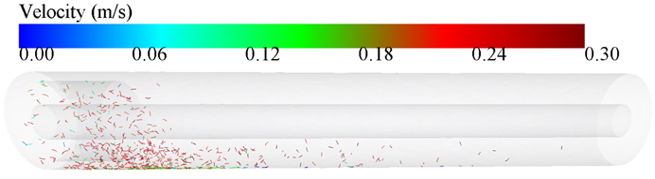
\includegraphics[width=\linewidth]{figure/iron-wire-distribution-1cp-velocity-colored.png} 
            \label{fig:viscosity_1.0}
        \end{minipage}
    }
    \vspace{0pt} % 上下两张图之间的垂直间距，可根据需要调整
    % --- 子图 (b) ---
    \subfloat[$\mu = 1.7\mathrm{mPa}\cdot\mathrm{s}$]{
        \begin{minipage}[t]{0.8\linewidth}
            \centering
            % 替换为你的第二张图片文件名
            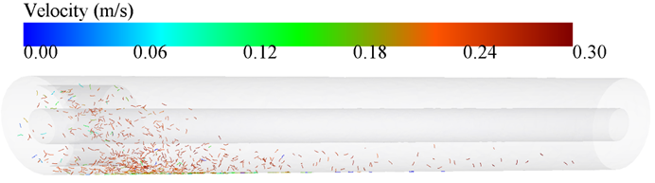
\includegraphics[width=\linewidth]{figure/iron-wire-distribution-1dot7-cp-velocity-colored.png} 
            \label{fig:viscosity_1.7}
        \end{minipage}
    }
    % --- 总标题 ---
    \caption{洗井液粘度对铁屑颗粒速度分布的影响（$\theta=90^\circ$,\ $v_{\mathrm{in}}=0.27\mathrm{m/s}$）}
    \label{fig:iron_wire_distribution_viscosity}
\end{figure}

图\ref{fig:iron_wire_mean_velocity_evolution_viscosity}为两种洗井液粘度下井筒稳态后铁屑颗粒沉积域铁屑颗粒运移速度图。从图中可以看出，$\mu$从$1.0\mathrm{mPa\cdot s}$增加到$1.7\mathrm{mPa\cdot s}$时，粘度增加到$1.7$倍，但铁屑的平均运移速度只增加到$1.04$倍，证明洗井液的粘度对铁屑运移的影响十分有限。
\begin{figure}[htbp]
    \centering
    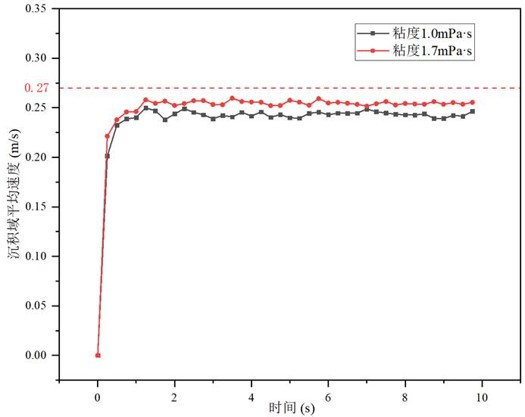
\includegraphics[width=0.7\textwidth]{figure/iron-wire-mean-velocity-evolution-viscosity.jpg}
    \caption{洗井液粘度对铁屑颗粒运移速度时间演变的影响（$\theta=90^\circ$,\ $v_{\mathrm{in}}=0.27\mathrm{m/s}$）}
    \label{fig:iron_wire_mean_velocity_evolution_viscosity}
\end{figure}

\subsection{洗井液流速对铁屑运移规律的影响}

本节探究洗井液流速对井筒环形空间内铁屑颗粒运移的影响。选取了水平段为研究对象，给定$\mu=1.7\mathrm{mPa\cdot s}$。

图\ref{fig:iron_wire_distribution_velocity}描述的是两种流速下井筒内铁屑颗粒分布情况，入口流速对铁屑颗粒运移行为的影响显著。铁屑的密度较大，在两种进口流速下，均表现出在边运移边沉积的现象，在水平管的底部位置有形成颗粒床的趋势。
随着洗井液流速的增加，从颗粒工厂出发的铁屑颗粒整体上产生了更大的轴向位移，颗粒整体的瞬时速度也有增加的趋势。这是由于洗井液流速增大时，铁屑颗粒受到流体沿轴向给予的拖拽力增加，铁屑颗粒沿轴向运移的速度增加。同时，增大的拖拽力也能对抗管壁摩擦效应，颗粒的运移效率增加。
\begin{figure}[htbp]
    \centering
    % --- 子图 (a) ---
    % 使用 minipage 控制宽度，这里设为 0.9\textwidth 让图片大一点
    % [t] 表示顶部对齐，防止因为图片高度不同导致错位
    \subfloat[$v_{\mathrm{in}} = 0.17\mathrm{m/s}$]{
        \begin{minipage}[t]{0.8\linewidth}
            \centering
            % 替换为你的第一张图片文件名
            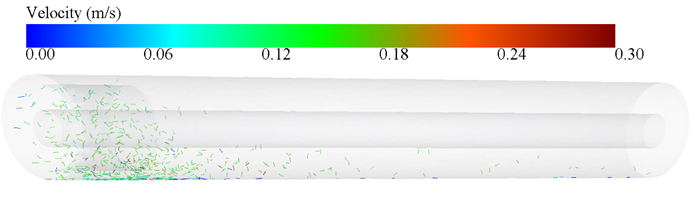
\includegraphics[width=\linewidth]{figure/iron-wire-distribution-1dot7cp-0dot17mpers.png} 
            \label{fig:distribution_velocity_0.17}
        \end{minipage}
    }
    \vspace{0pt} % 上下两张图之间的垂直间距，可根据需要调整
    % --- 子图 (b) ---
    \subfloat[$v_{\mathrm{in}} = 0.27\mathrm{m/s}$]{
        \begin{minipage}[t]{0.8\linewidth}
            \centering
            % 替换为你的第二张图片文件名
            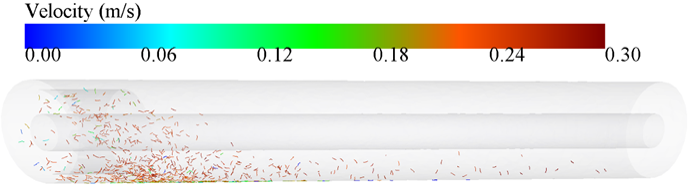
\includegraphics[width=\linewidth]{figure/iron-wire-distribution-1dot7cp-0dot27mpers.png} 
            \label{fig:distribution_velocity_0.27}
        \end{minipage}
    }
    % --- 总标题 ---
    \caption{洗井液流速对铁屑颗粒分布的影响（$\theta=90^\circ$,\ $\mu = 1.7\mathrm{mPa}\cdot\mathrm{s}$）}
    \label{fig:iron_wire_distribution_velocity}
\end{figure}

铁屑颗粒的运动迹线图直观地展现了颗粒的运动轨迹，本文选取了井筒内的部分铁屑颗粒，绘制了两种流速下其迹线图，如图\ref{fig:iron_wire_particle_track_velocity}所示。从图中可以看出，在颗粒工厂中产生的铁屑颗粒一经产生，将很快获得轴向移动速度，这一点可从左上至右下的迹线得到证明；且进口流速越大，迹线的斜率越小，颗粒获得的周向速度也越大。在两种情况下，颗粒落到管底后，以较大幅度弹跳的方式向前运动，而非形成密实的颗粒床以整体的形式运动。在图\ref{fig:distribution_velocity_0.27}中，铁屑颗粒在颗粒工厂右边界附近的迹线混叠密度也低于前者，说明进口流速提升时，颗粒得以弥散开来，颗粒床的形成受到了抑制。

%这两张图的总仿真时间是个很重要的变量。第一个总的仿真时间长，第二个总的仿真时间短。总仿真时间长，颗粒的运动轨迹就会更长，颗粒的运动轨迹就会更密集。总仿真时间短，颗粒的运动轨迹就会更短，颗粒的运动轨迹就会更稀疏。

\begin{figure}[htbp]
	\centering
	% --- 子图 (a) ---
	% 使用 minipage 控制宽度，这里设为 0.9\textwidth 让图片大一点
	% [t] 表示顶部对齐，防止因为图片高度不同导致错位
	\subfloat[$v_{\mathrm{in}} = 0.17\mathrm{m/s}$]{
		\begin{minipage}[t]{0.8\linewidth}
			\centering
			% 替换为你的第一张图片文件名
			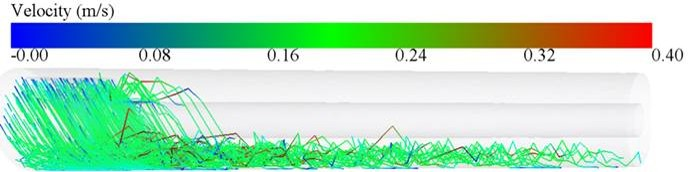
\includegraphics[width=\linewidth]{figure/iron-wire-particle-track-1dot7cp-0dot17mpers.jpg} 
			\label{fig:track_velocity_0.17}
		\end{minipage}
	}
	\vspace{0pt} % 上下两张图之间的垂直间距，可根据需要调整
	% --- 子图 (b) ---
	\subfloat[$v_{\mathrm{in}} = 0.27\mathrm{m/s}$]{
		\begin{minipage}[t]{0.8\linewidth}
			\centering
			% 替换为你的第二张图片文件名
			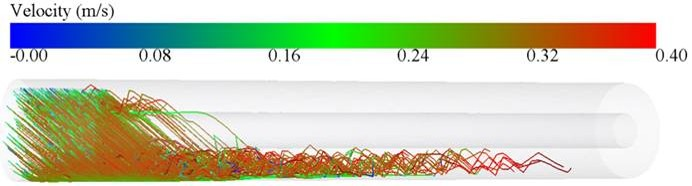
\includegraphics[width=\linewidth]{figure/iron-wire-particle-track-1dot7cp-0dot27mpers.jpg} 
			\label{fig:track_velocity_0.27}
		\end{minipage}
	}
	% --- 总标题 ---
	\caption{洗井液流速对铁屑颗粒分布的影响（$\theta=90^\circ$,\ $\mu = 1.7\mathrm{mPa}\cdot\mathrm{s}$）}
	\label{fig:iron_wire_particle_track_velocity}
\end{figure}

图\ref{fig:iron_wire_mean_velocity_evolution_incoming_velocity}给出了$v_{\mathrm{in}}=0.17\mathrm{m/s}$,\ $0.27\mathrm{m/s}$两种情况下铁屑颗粒在沉积域中运移速度定量结果。洗井液流动产生的携屑作用足以克服井筒内壁摩擦作用，沉积在井筒底部的铁屑形成移动铁屑床。颗粒的平均轴向运动速度是小于来流（平均）速度，这说明铁屑颗粒在井筒内的运移过程中，受到井壁摩擦力的影响。随着时间的推移，铁屑颗粒在沉积域中的平均运移速度逐渐趋于稳定，表明颗粒在井筒内的运移达到了动态平衡状态。随着洗井液流速的增加，井筒内沉积域铁屑颗粒运移速度也会大幅度增加，于是，洗井液的流速对铁屑运移有显著影响。
\begin{figure}[htbp]
	\centering
	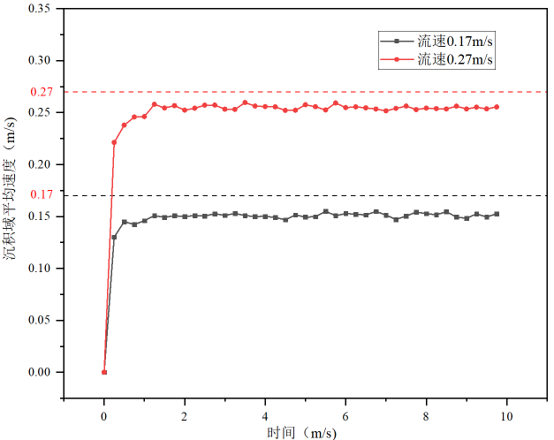
\includegraphics[width=0.7\textwidth]{figure/iron-wire-mean-velocity-evolution-incoming-velocity.png}
	\caption{洗井液速度对铁屑颗粒运移速度时间演变的影响（$\mu=1.7\mathrm{mPa\cdot s}$）}
	\label{fig:iron_wire_mean_velocity_evolution_incoming_velocity}
\end{figure}

\subsection{井斜对铁屑运移规律的影响}
本节将探究井斜对于井筒环形空间内铁屑颗粒运移的影响。选取了直井（$\theta = 0^\circ$）、45°斜井（$\theta = 45^\circ$）和水平井（$\theta = 90^\circ$）三种井斜，洗井液入口流速为$v_\mathrm{in}=0.27\mathrm{m/s}$，粘度取$\mu=1.7\mathrm{mPa\cdot s}$。

图\ref{fig:iron_wire_distribution_3angles}描述了不同井斜角度下井筒内铁屑颗粒瞬时分布情况。从图中可以看出，直井（$\theta = 0^\circ$）中井筒中铁屑不能向上迁移，目前的流体拖曳力不足以克服重力的作用。$\theta = 45^\circ$斜井中，铁屑床主要沉积在颗粒工厂附近的底部井壁上，距流体入口较近，流体出口附近几乎没有铁屑颗粒。$\theta = 90^\circ$的水平井，颗粒同样会聚集在井壁上，但颗粒床迁移的距离更远，聚集度更低，且出口处颗粒的数量比$\theta = 45^\circ$斜井中更多。
%$\theta = 45^\circ$和$\theta = 90^\circ$两种情况下，铁屑床都由移动床和静止床两部分组成，静止床的出现意味着上部铁屑积压，流体拖曳力、重力和摩擦作用相平衡；移动床的出现意味着流体的拖拽作用足以克服重力和管壁摩擦对单个铁屑颗粒的作用，使铁屑持续运移。表明，单个颗粒的行为有别于一群颗粒的行为，颗粒-颗粒之间的相互作用会影响颗粒的运移行为。
结合三种情况可以推测：第一，在直井中，作业产生的铁屑一定会下落至井底；第二，存在一个临界井斜$\theta_c$，当$\theta < \theta_c$时，铁屑颗粒会一直下落至井底形成堆积，而当$\theta > \theta_c$时，铁屑颗粒会在井筒壁面中形成堆积；第三，$\theta_c<45^\circ$，且其大小与流体的流速、粘度以及铁屑颗粒的密度、形状等因素相关。

\begin{figure}[htbp]
	\centering
	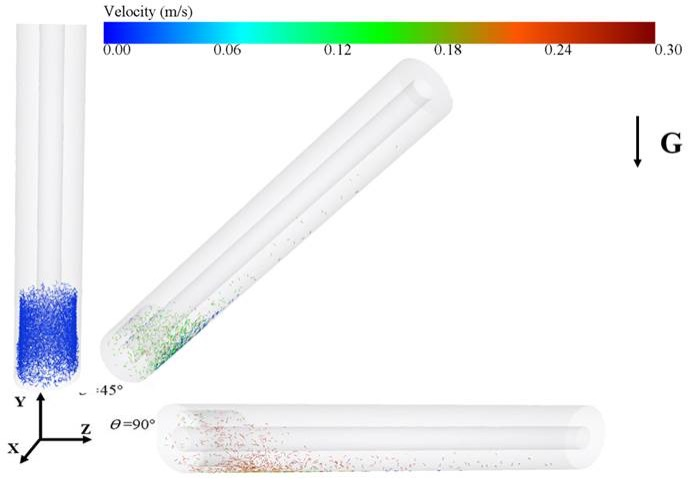
\includegraphics[width=0.7\textwidth]{figure/iron-wire-distribution-1dot7cp-0dot27mpers-3angles.jpg}
	\caption{井斜角对铁屑颗粒分布情况}
	\label{fig:iron_wire_distribution_3angles}
\end{figure}

铁屑颗粒的流动迹线图可以直观地描述颗粒的运动轨迹。首先选取井筒内的部分铁屑颗粒，绘制不同井斜角度下部分铁屑流动迹线图，如图\ref{fig:iron_wire_track_3angles}所示。直井（$0^\circ$）中铁屑运动轨迹平直，说明铁屑几乎不与井壁产生接触（或碰撞），短促的轨迹说明颗粒将向井底沉积，不能持续随流运移。各井斜条件下井壁处与颗粒工厂处的颗粒速度均较小，水平井环空内的颗粒速度大于斜井。这是由于井筒轴线与重力方向的夹角增大，环空中颗粒所受重力的影响愈发显著，颗粒在自身重力作用下下沉加快，洗井液在轴向上不足以提供足够的悬浮能量，颗粒堆积到底部后形成颗粒床，运移效率明显降低。

\begin{figure}[htbp]
	\centering
	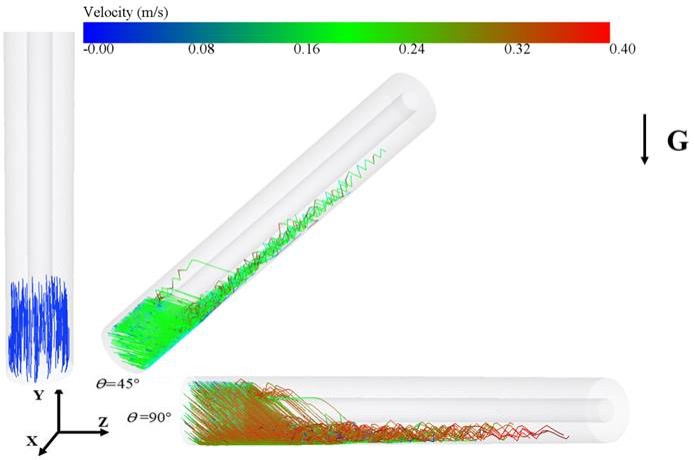
\includegraphics[width=0.7\textwidth]{figure/iron-wire-particle-track-1dot7cp-0dot27mpers-3angles.jpg}
	\caption{井斜角对铁屑运动轨迹的影响}
	\label{fig:iron_wire_track_3angles}
\end{figure}

斜井（$\theta = 45^\circ$）中移动铁屑床的平均运移速度小于水平井（$\theta = 90^\circ$），如图\ref{fig:iron_wire_velocity_3angles}所示。水平井中铁屑颗粒的运移速度接近环空平均流速，而斜井中铁屑颗粒的运移速度仅为环空平均流速的一半左右。

\begin{figure}[htbp]
	\centering
	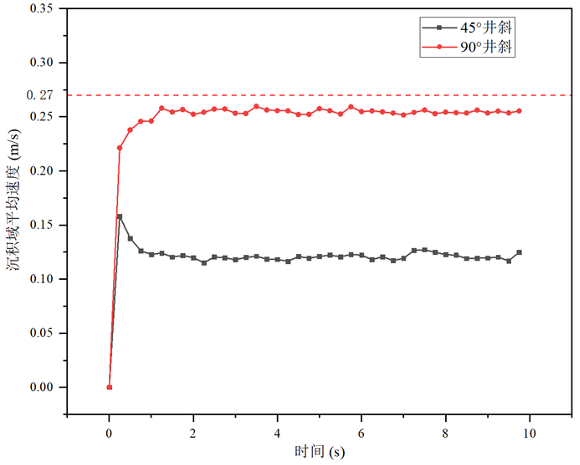
\includegraphics[width=0.7\textwidth]{figure/iron-wire-mean-velocity-evolution-3angles.png}
	\caption{井斜角对铁屑运动速度的影响}
	\label{fig:iron_wire_velocity_3angles}
\end{figure}

综合上述仿真结果可以发现，洗井液粘度增大和环空流速提高对铁屑颗粒的运移效率均有正向作用，因此选用更高粘度的洗井液、采用更大的洗井排量有助于铁屑颗粒从井筒中排出。但是，铁屑的运移行为受井筒倾角影响很大：在直井和小斜度井中，铁屑难以通过常规的洗井液循环方式排出，需开发具有\textbf{吸附}、\textbf{过滤}功能的\textbf{专用清洁工具}将铁屑从井筒中捞出。针对丝状铁屑的仿真结果可进一步推广至片状、块状铁屑等情形，此类高密度碎屑在井筒中的运移能力较差。

\section{井筒内结垢物运移及分布规律研究}
海上油井钡锶垢是由地层水与注入水（如海水）混合后，因钡（$\mathrm{Ba^{2+}}$）、锶（$\mathrm{Sr^{2+}}$）离子与硫酸根（$\mathrm{SO_4^{2-}}$）或碳酸根（$\mathrm{CO_3^{2-}}$）结合形成的难溶性无机盐（如硫酸钡、硫酸锶），在井筒、管道或设备表面沉积形成的坚硬垢层；其生成受高温高压、高矿化度及流动条件影响，易堵塞油流通道、加剧设备腐蚀，甚至因伴生放射性物质（如镭）带来安全与环保风险。
研究钡锶垢的运移规律在油井洗井中至关重要，通过明确垢颗粒的迁移和沉降特性，优化洗井工艺参数，高效清除井筒和近井地带的顽固垢层，避免二次堵塞或地层伤害，从而恢复油井产能并延长寿命；同时可预测垢的沉积风险，指导防垢措施以减少设备腐蚀和放射性污染，降低维护成本与环境危害，并为建立结垢动力学模型、开发新型洗井技术提供理论支撑，最终实现安全、经济、环保的油田开发目标。

建立两种尺寸不同的钡锶垢颗粒模型，如图\ref{fig:BaSr_particle}所示。通过调研钡锶垢的物理性质及性状，将其运移仿真参数列于表\ref{tab:basr_simulation_params}。

\begin{figure}[htbp]
    \centering
    % 子图 (a)
    \subfloat[钡锶垢实物]{%
        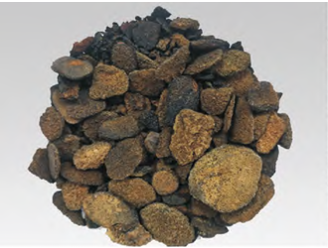
\includegraphics[width=0.48\linewidth]{figure/BaSr-sample.png}%
        \label{fig:BaSr_sample}%
    }
    \hfill
    % 子图 (b)
    \subfloat[SEM微观形貌]{%
        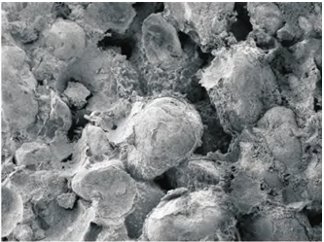
\includegraphics[width=0.48\linewidth]{figure/BaSr-SEM.png}%
        \label{fig:BaSr_SEM}%
    }
    \vspace{1em}
    % 子图 (c)
    \subfloat[垢仿真模型示意图]{%
        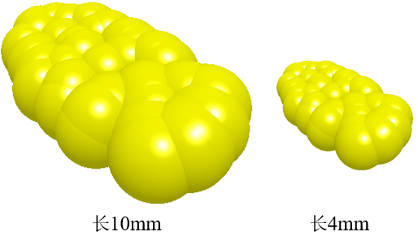
\includegraphics[width=0.5\linewidth]{figure/BaSr-model.png}%
        \label{fig:BaSr_model}%
    }
    \caption{钡锶垢颗粒及仿真模型对比}
    \label{fig:BaSr_particle}
\end{figure}

\begin{table}[htbp]
    \centering
    \caption{锁锶垢颗粒运移仿真参数}
    \label{tab:simulation_params}
    \begin{tabularx}{.9\textwidth}{cCCc}
        \toprule % 顶部粗线
        名称 & 符号 & 数值 & 单位 \\
        \midrule % 中间细线
        水平井筒长度 & $L$ & 1.5 & m \\
        井筒直径 & $D_H$ & 177.8 & mm \\
        钻杆直径 & $D_P$ & 88.9 & mm \\
        颗粒密度 & $\rho_P$ & 4336.0 & kg/m$^3$ \\
        洗井液密度 & $\rho_l$ & 1300.0 & kg/m$^3$ \\
        井斜角度 & $\theta$ & 0、45、90 & $^\circ$ \\
        洗井液入口流速 & $v_{in}$ & 0.37、0.59 & m/s \\
        洗井液粘度 & $\mu$ & 1.7 & mPa$\cdot$s \\
        沉积域距离井壁高度 & $H$ & 20.0 & mm \\
        颗粒与井壁静摩擦系数 & $\mu_s$ & 0.5 & - \\
        颗粒与井壁滑动摩擦系数 & $\mu_k$ & 0.4 & - \\
        \bottomrule % 底部粗线
    \end{tabularx}
\end{table}

\subsection{洗井液流速对钡锶垢运移规律的影响}

选取井斜$\theta = 45^\circ$，洗井液入口流速$V_{\mathrm{in}}$取$0.37\mathrm{m/s}$和$0.59\mathrm{m/s}$两种，洗井液粘度取$1.7\mathrm{mPa\cdot s}$，钡锶垢颗粒有两种尺寸，特征长度约为$10\mathrm{mm}$和$4\mathrm{mm}$。

图\ref{fig:Ba_Sr_distribution}描述的是不同洗井液流速下井筒内钡锶垢颗粒的分布情况，入口流速对钡锶垢颗粒运移效率的影响十分明显。随着洗井液流速增大，钡锶垢颗粒的运移速度逐渐增大。由于洗井液入口流速增大，产生于颗粒工厂的钡锶垢颗粒及悬浮层颗粒具有更大的轴向位移，在相同的仿真时间内，流速高时井筒内钡锶垢颗粒距离流体入口更远。
\begin{figure}[htbp]
	\centering
	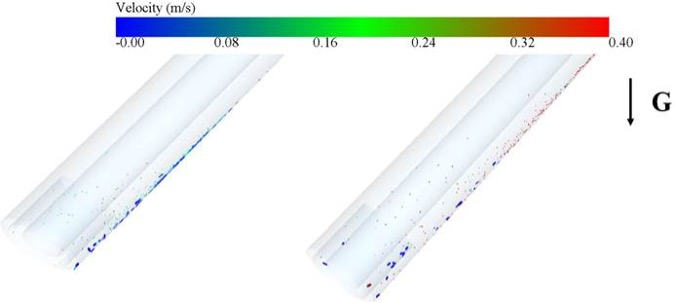
\includegraphics[width=0.7\textwidth]{figure/BaSr-distribution-Vin.jpg}
	\caption{钡锶垢颗粒在井筒中的运移}
	\label{fig:Ba_Sr_distribution}
\end{figure}

图\ref{fig:Ba_Sr_velocity_size}为钡锶垢在井筒洗井液流速$V_{\mathrm{in}}=0.37\mathrm{m/s}$和$V_{\mathrm{in}}=0.59\mathrm{m/s}$稳态后颗粒沉积域运移速度图。选取Z方向为竖直向上方向。$V_{\mathrm{in}}=0.37\mathrm{m/s}$时，大垢落到井壁上后会滑向井底，小垢在进入沉积域后会以远远低于井筒内流体的速度(约为$0.05\mathrm{m/s}$)缓慢向压力出口运移。$V_{\mathrm{in}}=0.59\mathrm{m/s}$时，大垢在进入沉积域之后Z方向速度几乎为零，少许的速度波动是由颗粒碰撞引起的，因此大垢在接触井壁后会在井壁上发生沉积现象，小垢在进入沉积域后会以低于井筒内流体的速度向压力出口运移，运移速度为$0.25\mathrm{m/s}$左右。

\begin{figure}[htbp]
	\centering
	\subfloat[$V_{\mathrm{in}}=0.37\mathrm{m/s}$]{%
	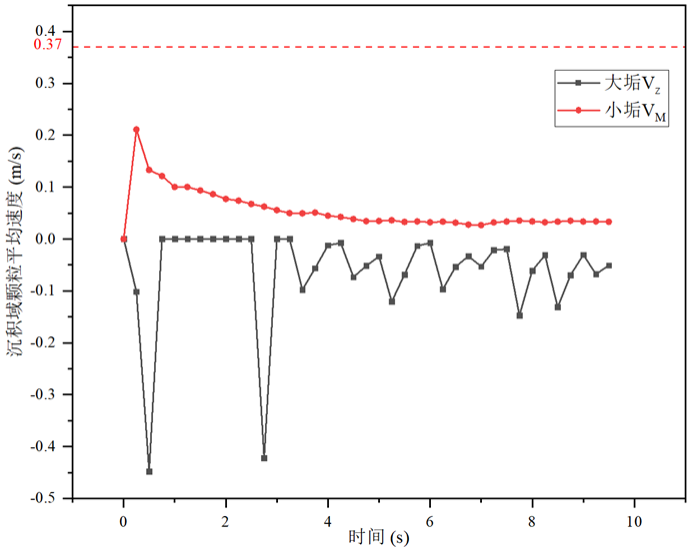
\includegraphics[width=0.48\textwidth]{figure/BaSr-mean-velocity-evolution-vin-dot37.png}
	}
	\subfloat[$V_{\mathrm{in}}=0.59\mathrm{m/s}$]{%
	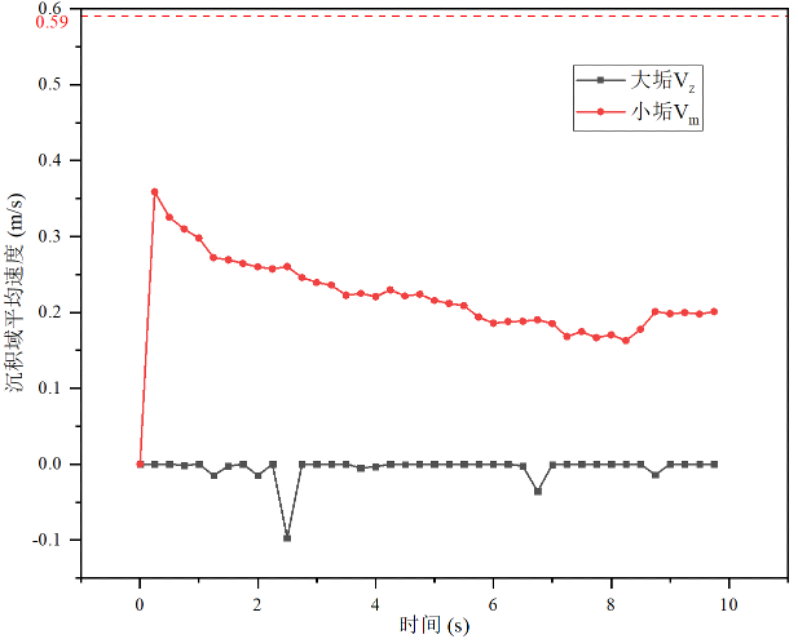
\includegraphics[width=0.48\textwidth]{figure/BaSr-mean-velocity-evolution-vin-dot59.png}
	}
	\caption{钡锶垢颗粒在沉积域运移平均速度演化}
	\label{fig:Ba_Sr_velocity_size}
\end{figure}

\subsection{井斜对钡锶垢运移规律的影响}

图\ref{fig:Ba_Sr_distribution_3angles}描述了井斜角变化时井筒内钡锶垢颗粒分布情况。$\theta=45^\circ$与$\theta=90^\circ$井斜下的钡锶垢颗粒都沉积在井底并以一定的速度向压力出口方向运移，其中$\theta=45^\circ$井筒内钡锶垢颗粒运移速度要大于$\theta=90^\circ$井筒内钡锶垢的运移速度，大颗粒钡锶垢在$\theta=45^\circ$与$\theta=90^\circ$井筒环空中均能够观察到，在直井（$\theta=0^\circ$）井筒环空中没有发现大颗粒钡锶垢，推测由于重力作用大颗粒钡锶垢产生后即下落至井底。而小颗粒钡锶垢运移速度随着井筒倾角的增大而减小，可见井筒倾角对钡锶垢运移效率有很大影响，其影响要以颗粒实际大小为准。

\begin{figure}[htbp]
	\centering
	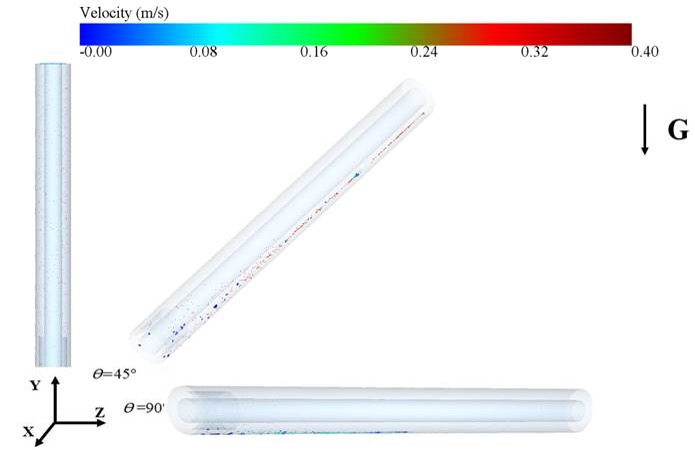
\includegraphics[width=0.7\textwidth]{figure/BaSr-distribution-3angles.jpg}
	\caption{钡锶垢颗粒在井筒中的运移}
\label{fig:Ba_Sr_distribution_3angles}
\end{figure}


图\ref{fig:Ba_Sr_velocity_3angles}(a)描述的是不同井斜下大颗粒钡锶垢井筒内运移速度变化，从图中可以看出，井斜45°与井斜90°情况下大颗粒钡锶垢因为重力影响在接触井壁后运移速度几乎为零，因此会在井壁产生沉积现场。井斜0°情况下大颗粒钡锶垢在井筒环空中运移，速度小于零说明大颗粒钡锶垢在以流体速度相反的方向运移，预测会在井底产生沉积。图\ref{fig:Ba_Sr_velocity_3angles}(b)描述的是不同井斜下小颗粒钡锶垢井筒内运移速度变化，从图中可以看出，随着井斜角的增加，钡锶垢在井筒内的运移速度逐渐减小。0°井斜下，钡锶垢在四秒左右即有颗粒到达压力出口，因为到达压力出口的钡锶垢颗粒速度减为0，随着越来越多的钡锶垢颗粒到达压力出口，其平均运移速度逐渐减小。45°与90°井斜下，钡锶垢颗粒由于重力作用在接触井筒内壁后会以一定速度向压力出口运移。由此可见，井斜可以明显影响钡锶垢颗粒的运移效率。

\begin{figure}[htbp]
	\centering
	\subfloat[$V_{\mathrm{in}}=0.37\mathrm{m/s}$]{%
	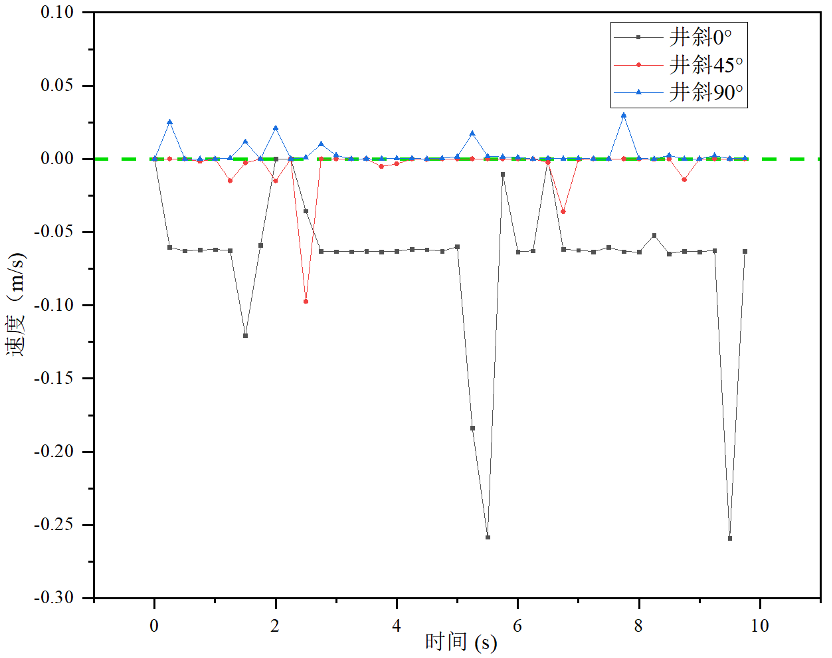
\includegraphics[width=0.48\textwidth]{figure/BaSr-mean-velocity-evolution-big-size.png}
	}
	\subfloat[$V_{\mathrm{in}}=0.59\mathrm{m/s}$]{%
	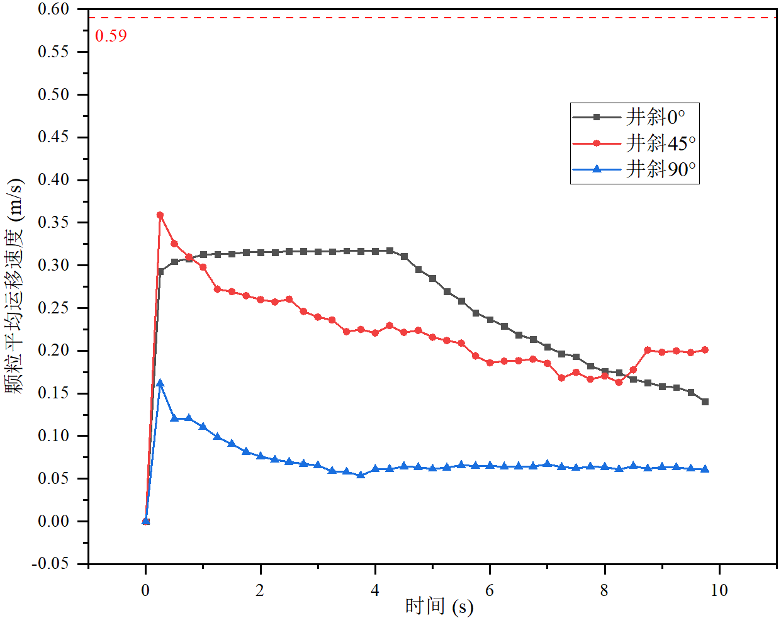
\includegraphics[width=0.48\textwidth]{figure/BaSr-mean-velocity-evolution-small-size.png}
	}
	\caption{钡锶垢颗粒在沉积域运移平均速度演化}
	\label{fig:Ba_Sr_velocity_3angles}
\end{figure}

仿真结果表明，洗井液流速增大时小钡锶垢颗粒的运移速度相应增大，因此在洗井作业中可适当提高洗井液流速以提升洗井效率。在流速0.59m/s的情况下，三种井斜工况下大钡锶垢颗粒均会发生沉积：0°井斜时沉积在井底，45°井斜时先沉积在井壁、随后向井底滑移，90°井斜时沉积在井壁，因此冲洗大块钡锶垢需要更高的泵送排量。在45°与90°井斜下，大小钡锶垢都会发生沉积，且小钡锶垢的运移速度远小于环空流体流速，因此在作业时应重点清洗斜井段与水平井段。

\section{井筒内蜡垢运移及分布规律研究}

油井中的蜡垢是原油中高碳链石蜡（$C_{18}$～$C_{60}$烃类）在开采过程中因温度、压力等条件变化析出并沉积形成的固态或半固态混合物，主要成分为石蜡、沥青质、胶质及机械杂质。其形成机制与原油组成和开采环境密切相关：当原油从高温高压地层流向井筒时，随着温度降低和压力释放，石蜡溶解度下降，逐步结晶析出并附着在管壁、泵阀等设备表面，形成致密垢层。蜡垢的危害显著：会堵塞油管导致产量下降，增加抽油能耗，加速设备磨损，甚至引发卡泵事故。
研究蜡垢运移规律对油井洗井过程至关重要，通过揭示蜡垢运移与沉积的动态机制，能够优化洗井参数，提升清蜡效率并降低井筒堵塞风险；在保障油井稳产、提高经济效益的同时，减少环境污染，推动油气开采的绿色高效发展。本节对蜡垢进行迁移仿真所用到的仿真条件如表\ref{tab:wax_params}所示。

\begin{table}[htbp]
    \centering
    \caption{蜡垢运移仿真参数}
    \label{tab:wax_params}
    \begin{tabularx}{.9\textwidth}{CCCC}
        \toprule % 顶部粗线
        名称 & 符号 & 数值 & 单位 \\
        \midrule % 中间细线
        水平井筒长度 & $L$ & 1.5 & m \\
        井筒直径 & $D_H$ & 177.8 & mm \\
        钻杆直径 & $D_P$ & 88.9 & mm \\
        颗粒密度 & $\rho_P$ & 800.0 & kg/m$^3$ \\
        洗井液密度 & $\rho_l$ & 1300.0 & kg/m$^3$ \\
        井斜角度 & $\theta$ & 0、45、90 & $^\circ$ \\
        洗井液入口流速 & $v_{in}$ & 0.37、0.59 & m/s \\
        洗井液粘度 & $\mu$ & 1.7 & mPa$\cdot$s \\
        沉积域距离井壁高度 & $H$ & 20 & mm \\
        颗粒模型大小 & - & 1、2、3、4 & mm \\
        颗粒与井壁静摩擦系数 & $\mu_s$ & 0.6 & - \\
        颗粒与井壁滑动摩擦系数 & $\mu_k$ & 0.2 & - \\
        \bottomrule % 底部粗线
    \end{tabularx}
\end{table}

\subsection{洗井液流速对蜡垢运移规律的影响}

本节改变洗井液流速，探究其对井筒环形空间内蜡垢颗粒运移的影响。取井斜45°，洗井液入口流速分别为0.37m/s、0.59m/s，粘度取$1.7\mathrm{mPa\cdot s}$，蜡垢颗粒粒径取2mm、4mm、6mm、8mm四种。

图1.41(a)描述了流体流速0.37m/s不同粒径下45°井筒内沉积域蜡垢颗粒平均速度情况，从图中可以看出，进入沉积域后蜡垢会以大于井筒内流体的速度向压力出口运移，随着粒径的增大，其运移速度也越来越大，并在四秒后蜡垢颗粒陆续到达压力出口。图1.41(b)描述了环空流体流速0.59m/s不同粒径下45°井筒内沉积域蜡垢颗粒平均速度情况，从图中可以看出，随着环空流体流速增大，蜡垢颗粒的运移速度也会增大，环空流体流速0.59m/s条件下，蜡垢颗粒在2.5秒后到达压力出口，相对于环空流体流速0.37m/s条件，蜡垢颗粒到达压力出口的速度变快。由此可见，环空流体流速对于蜡垢颗粒运移效率的影响显著。
\begin{figure}[htbp]
	\centering
	\subfloat[$V_{\mathrm{in}}=0.37\mathrm{m/s}$]{%
	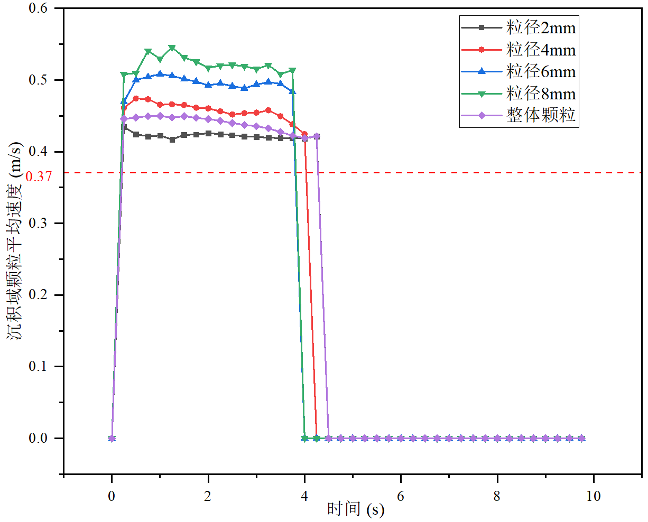
\includegraphics[width=0.48\textwidth]{figure/Wax-mean-velocity-Vin-dot37mpersec.png}
	}
	\subfloat[$V_{\mathrm{in}}=0.59\mathrm{m/s}$]{%
	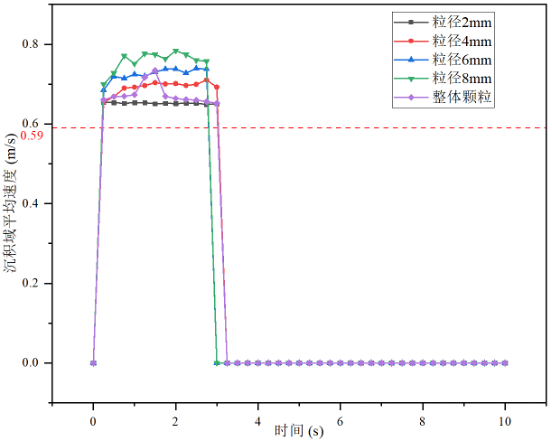
\includegraphics[width=0.48\textwidth]{figure/Wax-mean-velocity-Vin-dot59mpersec.png}
	}
	\caption{蜡垢颗粒在沉积域运移平均速度演化}
	\label{fig:Wax_velocity_particle_size}
\end{figure}

\subsection{井斜对蜡垢颗粒运移规律的影响}
本节改变井筒倾角，探究其对井筒环形空间内蜡垢颗粒运移的影响。选取井斜$\theta_c = 0^\circ$、45°、90°，洗井液入口流速为0.59m/s，粘度取$1.7\mathrm{mPa\cdot s}$，蜡垢颗粒粒径取2mm、4mm、6mm、8mm四种。图\ref{fig:wax_velocity_3angles}(a)描述了环空流体流速0.59m/s时0°井筒内不同粒径蜡垢颗粒在沉积域的平均速度变化情况：随着蜡垢颗粒粒径增大，其运移速度也增大，且均高于环空流体流速；在环空流体流速0.59m/s条件下，蜡垢颗粒在2.5s后到达压力出口。与45°井筒倾角工况相比，0°倾角井筒内蜡垢颗粒的最大运移速度更高，但其达到最大运移速度的时间长于45°井筒倾角工况。图\ref{fig:wax_velocity_3angles}(b)描述了环空流体流速0.59m/s时90°井筒内不同粒径蜡垢颗粒在沉积域的平均速度变化情况：随着蜡垢颗粒粒径增大，其运移速度反而减小，且均低于环空流体流速，可见摩擦力作用会导致蜡垢颗粒的运移速度下降；在环空流体流速0.59m/s条件下，蜡垢颗粒在4s后到达压力出口。与0°、45°井筒倾角工况相比，90°倾角井筒内蜡垢颗粒的最大运移速度明显下降，到达压力出口的时间变长，运移效率降低。


\begin{figure}[htbp]
	\centering
	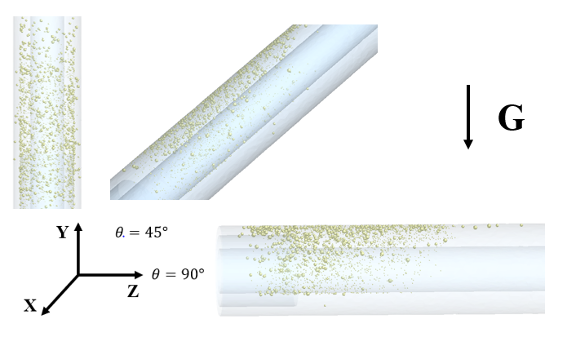
\includegraphics[width=0.7\textwidth]{figure/wax-distribution-3angles.png}
	\caption{不同井斜下蜡垢颗粒井筒内运移分布图}
\label{fig:wax_distribution_3angles}
\end{figure}


\begin{figure}[htbp]
	\centering
	\subfloat[$\theta=0^\circ$]{%
	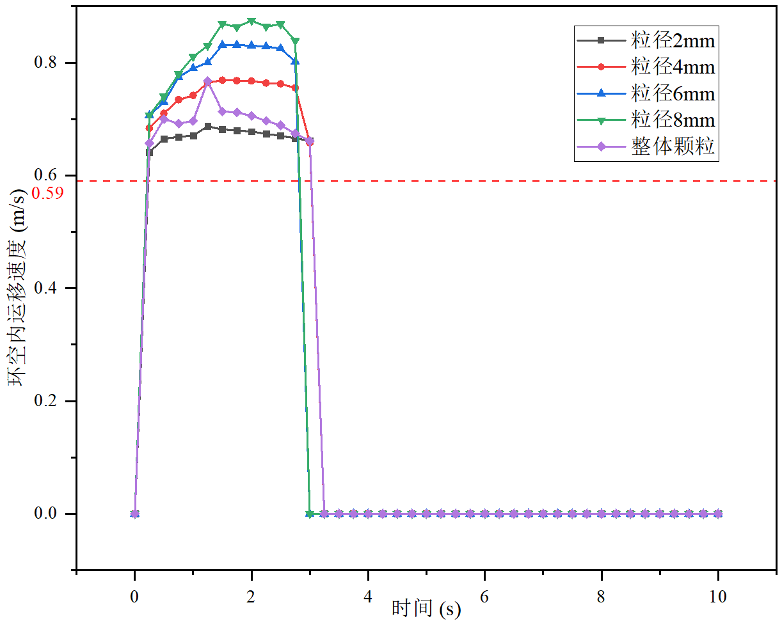
\includegraphics[width=0.48\textwidth]{figure/Wax-mean-velocity-Vin-dot59mpersec-theta-0.png}
	}
	\subfloat[$\theta=90^\circ$]{%
	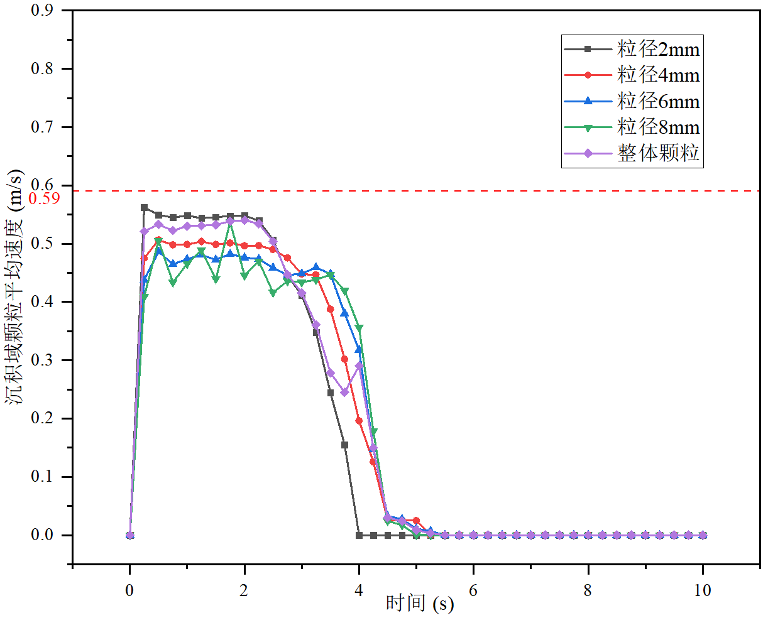
\includegraphics[width=0.48\textwidth]{figure/Wax-mean-velocity-Vin-dot59mpersec-theta-90.png}
	}
	\caption{井斜对蜡垢颗粒在沉积域运移平均速度演化的影响}
	\label{fig:wax_velocity_3angles}
\end{figure}

通过这些仿真发现，蜡垢颗粒的运移规律跟颗粒大小有关，在0°与45°井斜条件下，蜡垢颗粒的粒径越大，其运移速度越大。90°井斜条件下，蜡垢颗粒越小，其运移速度越大。随着井斜角度增加，蜡垢颗粒的运移速度也逐渐减小。 在各个井段并未发生蜡垢沉积现象。

\section{本章小结}

本章针对修井及洗井作业中砂砾、铁屑、结垢物（钡锶垢）和蜡质四类典型颗粒物在井筒内的运移及分布问题，基于流体动力学与颗粒动力学理论，建立了 EDEM--Fluent 双向耦合的液固两相流数值模拟方法，并以洗井液流速 $v_{\mathrm{in}}$、粘度 $\mu$ 和井斜角 $\theta$ 为核心控制变量，系统研究了四类颗粒在井筒环空内的运移轨迹、沉积速率及空间分布特征，主要结论如下：

（1）建立了井筒环空颗粒运移的 EDEM--Fluent 耦合仿真方法。颗粒相采用 Hertz--Mindlin 接触模型描述颗粒间以及颗粒与壁面间的接触、碰撞与摩擦作用，对含湿、存在液桥力的工况可采用 Hertz--Mindlin with JKR 接触模型；液固相间作用采用 Gidaspow 曳力模型，并计入 Saffman 剪切升力与 Magnus 旋转升力；液相采用 N--S 方程与标准 $k-\epsilon$ 湍流模型求解（部分工况采用 $SST\ k-\omega$ 模型），通过耦合接口实现颗粒运动与流场动量的双向传递。计算模型取长 $1.5$ m 的环空管段，模拟 $\phi 88.9$ mm 钻杆与 $\phi 244.475$ mm（$9$-5/8\inch）、$\phi 177.8$ mm（$7$\inch）井筒的组合工况，井斜角取 $0^\circ$、$45^\circ$、$90^\circ$，洗井液流速取 $0.17\sim0.69$ m/s，粘度取 $1.0\sim5.0\ \mathrm{mPa}\cdot\mathrm{s}$。

（2）基于现场砂样粒度分级统计结果（中砂 35.29\%、细砂 47.15\%、极细砂 13.99\%）建立了 9.9 万个不同粒径砂砾颗粒的仿真模型，获得了环空内砂砾的沉降与分布规律。钻杆静止时环空内砂砾质量在约 30 s 后趋于稳定，稳定沉积量平均约 $63.294$ kg；由于环空上部为流体高速区、下部为低速区，砂砾受重力作用大量沉降于环空下部低速区并形成砂床，砂砾床主要沉积在水平段，井斜角增大后井斜段内砂砾体积分数明显减小。随洗井液流速由 $0.17$ m/s 增至 $0.69$ m/s，砂床最高点（b 点）高度由 $68$ mm 降至 $32$ mm，且砂砾体积分数减小、砂砾流速增大，表明增大排量可增强流体携砂能力、降低砂堵风险；随洗井液粘度由 $1.0\ \mathrm{mPa}\cdot\mathrm{s}$ 增至 $5.0\ \mathrm{mPa}\cdot\mathrm{s}$，砂床最高点高度由 $77.5$ mm 降至 $25$ mm，但砂砾流速呈减小趋势，即增大粘度在提高携砂能力的同时会降低环空流体的流动性、延长砂砾上返时间。因此，工程上减小砂堵风险应以增大冲砂排量为主要手段，以适度提高洗井液粘度为辅。

（3）明确了颗粒在工具与井筒环空内沉积的“危险位置”。以外部功能单元最多、结构最复杂的“四合一”工具扶正器与强磁部位和 $7$\inch 井筒构成的环空为对象，在环空流速 $0.37$、$0.59$ m/s 下开展仿真，结果表明部分砂砾会因重力作用在工具前端产生堆积，并在强磁部件的凹槽内少量滞留；环空流速增大后颗粒的轴向位移与运移效率明显提高。工具的导流结构可引导砂砾随流运移，与增大冲砂排量相配合能够有效降低砂堵概率，为工具安全作业提供保障。

（4）揭示了铁屑颗粒“粘度弱敏感、流速强敏感、井斜角决定性”的运移规律。以井下封隔器套铣作业返出碎屑中的丝状铁屑（密度 $7800$ kg/m$^{3}$）为典型建模对象：颗粒在沉积域中的平均轴向速度始终小于来流平均速度，表明井壁摩擦对颗粒运移具有显著阻滞作用，随时间推移运移速度逐渐趋于稳定，颗粒运移达到动态平衡状态；粘度由 $1.0\ \mathrm{mPa}\cdot\mathrm{s}$ 增至 $1.7\ \mathrm{mPa}\cdot\mathrm{s}$（增至 $1.7$ 倍）时，沉积域内颗粒的平均运移速度仅增至 $1.04$ 倍，说明洗井液粘度对铁屑运移的影响十分有限；流速由 $0.17$ m/s 增至 $0.27$ m/s 时，颗粒的轴向位移与瞬时速度大幅提高，颗粒床的形成受到抑制，说明流速是铁屑运移最敏感的控制因素；井斜角的影响最为显著，直井（$\theta=0^\circ$）中流体拖曳力不足以克服重力，铁屑不能上返、必然下落至井底；$45^\circ$ 斜井中铁屑床堆积在靠近颗粒工厂一侧的底部井壁，出口附近几乎没有颗粒；水平井（$\theta=90^\circ$）中颗粒床迁移距离更远、聚集度更低、出口处颗粒数量更多，但移动铁屑床的平均运移速度仅约为环空平均流速的一半。据此推测存在临界井斜角 $\theta_c<45^\circ$：当 $\theta<\theta_c$ 时铁屑一致下落至井底形成堆积，当 $\theta>\theta_c$ 时铁屑在井壁堆积。上述结论可推广至片状、块状等高密度金属屑。可见在直井与小斜度井中，铁屑难以通过常规洗井液循环排出井筒，必须依靠具备\textbf{吸附}、\textbf{过滤}功能的\textbf{专用清洁工具}。

（5）阐明了结垢物（钡锶垢）颗粒的运移与沉积特征。以密度 $4336$ kg/m$^{3}$、特征长度分别约为 $10$ mm 和 $4$ mm 的两种钡锶垢颗粒为对象：随洗井液流速由 $0.37$ m/s 增至 $0.59$ m/s，垢颗粒的运移速度与轴向位移均增大；但在 $0.59$ m/s 时，三种井斜工况下的大颗粒垢均发生沉积，$0^\circ$ 井斜沉积于井底，$45^\circ$ 井斜先沉积于井壁继而向井底滑移，$90^\circ$ 井斜沉积于井壁；小颗粒垢的运移速度远低于环空流体流速（$0.37$ m/s 时约为 $0.05$ m/s、$0.59$ m/s 时约为 $0.25$ m/s），且随井斜角增大而减小；$45^\circ$ 与 $90^\circ$ 井斜下大小垢颗粒均会发生沉积。因此洗井作业时应重点清洗斜井段与水平井段，清除大块钡锶垢需要更高排量的水泵。

（6）明确了蜡垢颗粒的运移规律。蜡垢密度（$800$ kg/m$^{3}$）低于洗井液密度，在各计算工况下均未发生沉积。洗井液流速由 $0.37$ m/s 增至 $0.59$ m/s 时，颗粒运移速度增大，到达压力出口的时间由约 $4$ s 缩短至约 $2.5$ s；粒径与运移速度的关系随井斜角发生反转，$0^\circ$ 与 $45^\circ$ 井斜条件下粒径越大运移速度越大，$90^\circ$ 井斜条件下因井壁摩擦作用粒径越大运移速度反而越小；总体而言，随井斜角度增加蜡垢颗粒的运移速度逐渐减小。可见提高环空流速是改善蜡垢携带效果的有效途径。

需要指出的是，上述四类颗粒的仿真均在同心环空、光滑管壁、颗粒形状简化的条件下完成，未计入偏心环空、颗粒团聚、颗粒与工具全尺寸结构的相互作用以及地层非稳态出砂供给等因素，因此所得定量结果（如环空内沉积砂砾质量、砂床最高点高度、颗粒运移速度等）反映的是各工况下颗粒运移的规律性趋势，尚需通过室内物理模拟实验进一步检验，并逐步推广至偏心环空和更接近现场的多因素耦合工况。

综合本章研究可以看出，环空流体流速对砂砾、铁屑、钡锶垢和蜡质运移的控制作用最强，洗井液粘度的影响次之且对铁屑等高密度金属屑十分有限，而井斜角往往决定颗粒能否被携带出井筒；四类颗粒均倾向于在环空下部低速区或井壁处富集并形成颗粒床，仅依靠常规洗井液循环无法解决连续砂床、铁屑和顽固垢层在井筒内的残留问题。这既揭示了井筒清洁作业中砂堵、卡钻及工具失效风险的来源，也为后续开展室内颗粒运移实验、明确影响运移效果的主控因素，进而开发高效井筒清洁工具提供了理论依据。
